% AdaBioQPSO Manuscript
% Extends BioQPSO (preprint: https://www.researchsquare.com/article/rs-9178752/v1)
%
\documentclass[runningheads]{llncs}
%
\usepackage[T1]{fontenc}
\usepackage{graphicx}
\usepackage{algorithm}
\usepackage{orcidlink}
\usepackage{algpseudocode}
\usepackage{amsmath}
\usepackage{booktabs}
\usepackage{longtable}
\usepackage{amssymb}
\usepackage{url}
%
\begin{document}
%
\title{AdaBioQPSO: Adaptive Attractor Weight Scheduling for Hybrid
Quantum-Behaved Bio-Swarm Optimization}
%
\author{
Manav\inst{1}\orcidlink{0009-0005-5197-5195}
%\and
%Richa Bhatia\inst{2}
}
%
%\authorrunning{Manav et al.}
\authorrunning{Manav}
%
\institute{
Student, Department of Electronics and Communication Engineering,\\
Netaji Subhas University of Technology, Delhi, India\\
\email{manav-ug23@nsut.ac.in}
%\and
%Associate Professor, Department of Electronics and Communication Engineering,\\
%Netaji Subhas University of Technology, Delhi, India\\
%\email{richa.bhatia@nsut.ac.in}
}
%
\titlerunning{AdaBioQPSO: Adaptive Attractor Weight Scheduling}
\maketitle
%
% -----------------------------------------------------------------------
% ABSTRACT
% -----------------------------------------------------------------------
\begin{abstract}
Fixed attractor weights in BioQPSO cannot adapt to the shifting
exploration--exploitation balance during optimization. This paper
proposes AdaBioQPSO, which dynamically schedules the bio-leader
weight $\phi_3(t)$ in the three-term quantum attractor while
preserving $\phi_1+\phi_2+\phi_3=1$. Four strategies are introduced
and evaluated on ten classical benchmarks ($D\!\in\!\{30,50,100\}$,
30 runs) and feature selection on three UCI datasets against ten
algorithms including GWO and WOA. On Levy, FeedbackAda achieves
$1.90\times10^{-9}$---over seven orders of magnitude better than
fixed-weight AntBioQPSO ($1.33\times10^{-1}$); QPSO independently
achieves $6.49\times10^{-13}$ on the same function, so the claim is
\emph{relative to the fixed BioQPSO baseline}, not absolute. LinearAda
and CosineAda yield statistically significant improvements over QPSO
on Styblinski--Tang ($p\!=\!0.032$, $p\!=\!0.035$). CosineAda matches
94.83\% two-feature accuracy on Wisconsin Breast Cancer; PerParticleAda
achieves the best Ionosphere accuracy (93.02\%). Gains are
problem-dependent: Schwefel remains a shared weakness consistent with
the No-Free-Lunch theorem. FeedbackAda is recommended for smooth and
structured multimodal landscapes; CosineAda for oscillatory landscapes.

\keywords{Quantum-behaved particle swarm optimization \and
Adaptive weight scheduling \and Bio-inspired intelligence \and
Metaheuristic optimization \and Feature selection \and
Statistical comparison}
\end{abstract}

% -----------------------------------------------------------------------
% 1. INTRODUCTION
% -----------------------------------------------------------------------
\section{Introduction}

PSO models the collective behavior of a bunch of particles exploring a multidimensional search space, where each particle updates its movement based on both its own best-found position and the best position discovered by the swarm. Although it is widely used, the traditional PSO approach tends to suffer from
premature convergence and reduced diversity on multimodal functions.
Whereas QPSO, which was introduced by Sun
et al.~\cite{Sun2004}, addresses these limitations by modeling
particles as quantum entities in a delta potential well, replacing
explicit velocity vectors with probabilistic position sampling from
the corresponding probability density function. It eliminates the
velocity parameter, reduces the control parameter count, and achieves
strong global search behavior. Numerous hybrid QPSO variants have
since been proposed~\cite{Fallahi2022,wiley2023improvedqpso}, coupling
QPSO with deep learning~\cite{Patel2025}, adaptive topologies, and
bio-inspired operators.

In prior work~\cite{Manav2026BioQPSO}, we proposed BioQPSO, a hybrid
framework that embeds bio-inspired neighborhood guidance
\emph{directly} into the QPSO quantum attractor, yielding a
\emph{three-term weighted attractor}:
\begin{equation}
q_{i,d}(t) = \phi_1\,p_{i,d}(t) + \phi_2\,g_{d}(t) +
\phi_3\,b_{i,d}(t), \quad \phi_1 + \phi_2 + \phi_3 = 1,
\label{eq:bioqpso-attractor-recap}
\end{equation}
where $b_{i,d}(t)$ is a bio-dependent local leader drawn from either
pheromone-guided ant behavior (AntBioQPSO) or fitness-based bee
behavior with scout reinitialization (BeeBioQPSO). The framework was
validated on ten standard benchmark functions and a real-world feature
selection task, where BeeBioQPSO achieved 94.83\% accuracy using only
2 features on the Wisconsin Breast Cancer dataset.

A key limitation of BioQPSO is that the attractor weights
$\phi_1, \phi_2, \phi_3$ are \emph{fixed} throughout the run. This
is suboptimal because the relative utility of exploration versus
exploitation changes over the course of optimization: early
iterations benefit from strong neighborhood diversity (higher
$\phi_3$), while later iterations require focused convergence around
the global attractor (lower $\phi_3$). Static weights cannot
accommodate this shift.

This paper addresses that limitation by proposing
\textbf{AdaBioQPSO}, in which $\phi_3$ is dynamically scheduled
across the run while $\phi_1$ and $\phi_2$ are adjusted proportionally
to preserve the $\phi_1 + \phi_2 + \phi_3 = 1$ constraint. Four
scheduling strategies are introduced: (i)~\emph{LinearAda}, a simple
monotone decay from $\phi_3^{\max}$ to $\phi_3^{\min}$;
(ii)~\emph{CosineAda}, a smooth cosine-annealed schedule offering
gradient-free oscillation control; (iii)~\emph{FeedbackAda}, a
closed-loop strategy that increases $\phi_3$ upon detecting global
best stagnation and decreases it upon improvement; and
(iv)~\emph{PerParticleAda}, a fine-grained strategy that adjusts
$\phi_3$ independently per particle based on its individual stagnation
counter.

\paragraph{Why adapt $\phi_3$ rather than $\beta$ or all weights?}
Prior adaptive QPSO work~\cite{Fallahi2022} schedules the
contraction--expansion coefficient $\beta$, which controls the
\emph{step size} of quantum sampling. AdaBioQPSO instead modulates
$\phi_3$, which controls \emph{which attractor} (personal, global, or
bio-leader) guides each update---a mechanism unique to BioQPSO's
neighborhood leadership through pheromone or fitness rings. Scheduling
$\phi_3$ therefore complements, rather than duplicates, the $\beta$
decay already present in all QPSO-based methods, and confines
adaptivity to the bio-component that fixed-weight BioQPSO left
static~\cite{Manav2026BioQPSO}. Joint adaptation of all three weights
$\phi_1,\phi_2,\phi_3$ is deferred to future work (Section~\ref{sec:conclusion}).

\paragraph{Contributions.}
This paper makes the following contributions:
\begin{enumerate}
  \item Four principled $\phi_3$ scheduling strategies (LinearAda,
        CosineAda, FeedbackAda, PerParticleAda) built on the existing
        BioQPSO framework, each targeting a distinct scheduling
        hypothesis.
  \item A complexity-aware empirical study under identical budgets
        against ten algorithms including modern baselines GWO and WOA.
  \item Extended statistical validation: Friedman test, Holm-corrected
        pairwise Wilcoxon, average ranks, and rank-biserial effect
        sizes across all ten benchmarks.
  \item Ablation of the $4{:}3$ redistribution rule and FeedbackAda
        hyperparameters, plus scalability results at
        $D\!\in\!\{30,50,100\}$.
  \item Multi-dataset feature selection on Wisconsin Breast Cancer,
        Wine, and Ionosphere UCI datasets, confirming that adaptive
        scheduling preserves feature parsimony.
\end{enumerate}

The rest of the paper is structured as follows. Section~2 reviews
related work. Section~3 presents the methodology and complexity
analysis. Section~4 reports experiments, ablations, and statistical
tests. Section~5 covers sensitivity analysis. Section~6 discusses
limitations. Section~7 concludes.

% -----------------------------------------------------------------------
% 2. RELATED WORK
% -----------------------------------------------------------------------
\section{Related Work}

Research in swarm intelligence has produced a broad family of hybrid
and adaptive variants motivated by the limitations of classical
PSO---particularly susceptible to premature convergence, slow
fine-tuning on multimodal landscapes, and fixed control parameters
that cannot respond to evolving search dynamics.

\paragraph{Particle Swarm Optimization and its limitations.}
Kennedy and Eberhart's original PSO~\cite{Eberhart1995} simulates
social foraging behavior through velocity and position updates, driven
by personal and global best positions. Despite its widespread
adoption, classical PSO suffers from two well-documented failures
modes: premature convergence on multimodal landscapes, where the
swarm collapses around a suboptimal attractor before sufficient
exploration, and slow fine-tuning in later iterations, where the
inertia velocity term prevents precise local search. Li et
al.~\cite{Li2014} characterized these failure modes in terms of
network topology, showing that the global best topology amplifies
premature convergence relative to ring topologies. These findings
directly motivate neighborhood-guided hybrids such as the one
proposed here.

\paragraph{Recent metaheuristic optimizers.}
Grey Wolf Optimizer (GWO)~\cite{Mirjalili2014} and Whale Optimization
Algorithm (WOA)~\cite{Mirjalili2016} represent widely cited
nature-inspired baselines for continuous optimization. Large-scale and
hybrid variants---including salp-based GWO for feature
selection~\cite{Elgamal2020LSGWO}---demonstrate continued interest in
bio-swarm hybrids for high-dimensional search. More recent proposals
include the Secant Optimization Algorithm~\cite{Ibrahim2026SOA}, which
achieves competitive benchmark results without gradient information,
and the Schr\"odinger optimizer~\cite{Hussein2025SRA}, which couples
quantum-wave duality with stochastic search. Recent zoo-inspired
metaheuristics---the Stoat Optimization
Algorithm~\cite{Dehghani2024Stoat}, Bighorn Sheep Optimization
Algorithm~\cite{Dehghani2024Bighorn}, and Cape Lynx
Optimizer~\cite{Dehghani2024CapeLynx}---extend the family of
nature-inspired strategies, though none directly address the
exploration--exploitation scheduling problem considered here.
AdaBioQPSO is positioned as a \emph{scheduling extension} of an
existing QPSO hybrid rather than a new search metaphor; comparisons
against GWO and WOA test whether $\phi_3$ adaptation remains
competitive with modern swarm baselines under identical budgets.

\paragraph{Quantum-Behaved PSO.}
Sun et al.~\cite{Sun2004} replaced the deterministic velocity update
of PSO with a quantum-mechanical position update derived from the
Schr\"odinger equation for a delta potential well. The resulting
QPSO eliminates the velocity vector, reducing the parameter
count to a single contraction-expansion coefficient $\beta$ while
achieving provably global convergence under mild conditions. Fang et
al.~\cite{Fang2010} provide a comprehensive review of QPSO variants,
documenting consistent improvements over classical PSO on unimodal
and low-dimensional multimodal functions. However, they also note that QPSO's reliance on the global best attractor makes it
susceptible to premature collapse on highly multimodal landscapes
where the global best is misleading early in the run. Fallahi and
Taghadosi~\cite{Fallahi2022} demonstrated that feedback-driven
scheduling of $\beta$ substantially improves QPSO's multimodal
performance, and Zhang and Shi~\cite{Zhang2023} coupled QPSO with
reinforcement learning for path planning, extending the framework to
dynamic environments. These developments establish QPSO as a
competitive backbone for hybridization, but leave open the question
of how to complement its global attractor with the local neighborhood
intelligence.

\paragraph{Adaptive weight scheduling in PSO and QPSO.}
Linearly decreasing inertia weight was among the earliest adaptive
strategies for PSO~\cite{Eberhart1995}, providing more exploration
early and exploitation late. Yao et al.~\cite{Yao2024} extended this
with HSPSO, which integrates adaptive weight adjustment, reverse
learning, Cauchy mutation, and the Hook--Jeeves strategy, achieving
state-of-the-art results on the CEC-2005 and CEC-2014 suites and
on feature selection for the UCI Arrhythmia dataset. Adaptive
strategies for the contraction-expansion coefficient $\beta$ in QPSO
have similarly been proposed~\cite{Fallahi2022}, with
feedback-driven schedules outperform fixed decays on multimodal
benchmarks. A recurring finding across this literature is that no
single fixed schedule dominates across problem classes; the
exploration--exploitation trade-off is inherently
problem-dependent~\cite{Li2014}, which motivates systematic
comparison of scheduling strategies rather than advocacy of any
single one. The present work applies this lesson to the bio-leader
weight $\phi_3$ in the three-term attractor of BioQPSO, a parameter
absent from standard QPSO entirely.

\paragraph{Bio-inspired hybridization of PSO and QPSO.}
Karaboga's Artificial Bee Colony~\cite{Karaboga2005} partitions the
population into employed, onlooker, and scout roles, achieving strong
local exploitation through neighborhood search and global diversity
through scout reinitialization. The scout mechanism, in particular, has
proven effective at escaping stagnation, a property that carries over
directly to BeeBioQPSO's scout phase~\cite{Manav2026BioQPSO}. Ant
Colony Optimization, originally designed for combinatorial
problems~\cite{Das2009}, was extended to continuous domains through
Gaussian kernel-based archive sampling (ACO$_\mathcal{R}$), where
pheromone concentration guides which archive solutions exert stronger
influence---the same principle underlying AntBioQPSO's
pheromone-guided local leader selection. Lu et
al.~\cite{Lu2008} demonstrated that coupling QPSO with neighborhood
clustering improves search diversity on multimodal benchmarks,
foreshadowing the ring-topology neighborhood used in BioQPSO.
Yang~\cite{Yang2008} surveys a broader class of nature-inspired
metaheuristics and establishes the theoretical basis for why
multi-paradigm hybridization---combining quantum, ant, and bee
mechanisms---can produce algorithms more robust than any single
constituent.
\paragraph{Metaheuristic optimization for real-world classification tasks.}
Beyond benchmark functions, metaheuristic algorithms have
demonstrated practical value in feature selection and biomedical
classification. Hybrid optimizers have been applied to gene
expression-based diagnosis of primary Sj\"ogren's syndrome~\cite{Reviewer2026Sjogren},
Wilms tumor~\cite{Reviewer2026Wilms}, breast-cancer
subtyping~\cite{Reviewer2026BreastMiRNA}, and non-small-cell lung
cancer biomarker discovery~\cite{Reviewer2026NSCLC}. Alzubi et
al.~\cite{Alzubi2022ClusterComp} jointly optimized SVM
hyperparameters and feature weights using Harris Hawks Optimization
for Android malware detection, achieving state-of-the-art detection
rates and illustrating that swarm-driven feature selection
substantially reduces model complexity. The same group later coupled
Quantum Mayfly Optimization with an encoder-decoder LSTM for malware
classification~\cite{Alzubi2023MNA} and applied a Salp Swarm Algorithm
to optimize a multilayer perceptron for IoT intrusion
detection~\cite{Alzubi2024NEM}, reporting accuracy above 97\% across
three independent benchmarks. Movassagh et al.~\cite{Movassagh2023JAIHC}
showed that integrating invasive weed optimization with differential
Evolution for ANN training consistently outperforms stand-alone
metaheuristics, reinforcing the case for multi-paradigm
hybridization. Large-scale salp-based grey wolf optimization has
similarly been applied to feature selection and global
optimization~\cite{Elgamal2020LSGWO}. Alzubi et al.~\cite{Alzubi2025AEJ} extended this line to
feature-weighted classification, demonstrating that swarm-driven
selection significantly reduces model complexity without sacrificing
accuracy. These works collectively establish that bio-swarm mechanisms
are particularly effective when the search objective couples
classification accuracy with feature parsimony---exactly the setting
used to validate BioQPSO and, in this work, AdaBioQPSO.
\paragraph{BioQPSO: the direct predecessor.}
Manav~\cite{Manav2026BioQPSO} proposed BioQPSO, a hybrid framework
that extends the standard two-term QPSO attractor with an explicit
bio-inspired neighborhood guidance term weighted by $\phi_3$:
\begin{equation}
    q_{i,d}(t) = \phi_1\, p_{i,d}(t) + \phi_2\, g_d(t) +
    \phi_3\, b_{i,d}(t), \quad \phi_1+\phi_2+\phi_3=1.
\end{equation}
Two variants were proposed: AntBioQPSO, which selects the bio-leader
$b_{i,d}(t)$ as the ring-neighbor with the highest pheromone
concentration, and BeeBioQPSO, which selects the fittest ring-neighbor
and reinitializes stagnating particles as scouts. Evaluated on ten
standard benchmark functions (D=30, 30 runs) and a real-world feature
selection task on the Wisconsin Breast Cancer dataset, BioQPSO
demonstrated problem-dependent advantages over PSO, QPSO, ACO, and
ABC on the Wisconsin Breast Cancer feature-selection task, achieving
94.83\% classification accuracy using only two features. Sensitivity
analysis confirmed that the key hyperparameters ($\rho$, $\Delta$, $L$,
$\phi_3$) are robust to reasonable variation, with default values
generalizing well across benchmark types.

A limitation acknowledged by BioQPSO is that $\phi_3$ is held fixed
throughout the run. In early iterations, when the population is
diverse, and bio-leaders carry meaningful local information, a larger
$\phi_3$ amplifies exploration. In late iterations, when the swarm
has converged, and bio-leaders tend to cluster near the same
attractor, a reduced $\phi_3$ avoids redundant local guidance and
allows $\phi_2$ to drive final convergence. No principled mechanism
for adapting $\phi_3$ was proposed or evaluated.

\paragraph{Gap addressed by this work.}
Prior hybrid BioQPSO variants fix the bio-component weight throughout
the run, limiting their ability to balance early-stage diversity with
late-stage convergence. AdaBioQPSO fills this gap by (i)~scheduling
$\phi_3$ via four strategies; (ii)~ablation of scheduling components
and the $\phi_1{:}\phi_2$ redistribution rule; (iii)~comparison
against classical \emph{and} modern baselines (GWO, WOA); and
(iv)~scalability, multi-dataset feature selection, and extended
statistical testing beyond QPSO-only Wilcoxon comparisons.

% -----------------------------------------------------------------------
% 3. METHODOLOGY
% -----------------------------------------------------------------------
\section{Methodology}

\subsection{Experimental Assumptions}

To maintain consistency, all simulations adopt the following
assumptions as taken in the prior research ~\cite{Manav2026BioQPSO} : (i)~all benchmark functions are formulated as minimization problems in $D = 30$ dimensions; 
(ii)~particle positions are uniformly randomly initialized within the predefined search space bounds; 
(iii)~each algorithm is executed over 30 independent trials, using a swarm size of 30 particles and 1000 iterations per run; 
(iv)~the contraction--expansion parameter $\beta$ in QPSO-based methods is linearly reduced from 1.0 to 0.5 throughout the optimization process; 
(v)~identical random seeds are employed across all algorithms to ensure fair and consistent statistical comparison; and 
(vi)~no external datasets are utilized, as all benchmark data are generated synthetically via simulation.

\subsection{BioQPSO Framework (Recap)}

AdaBioQPSO is built on the BioQPSO framework proposed
in~\cite{Manav2026BioQPSO}. We briefly recap the key components for
self-containedness.

\paragraph{QPSO position update.}
Each particle is modeled as a quantum entity in a delta potential
well~\cite{Sun2004,Fang2010}. Its position is sampled as:
\begin{equation}
x_{i,d}(t+1) =
\begin{cases}
q_{i,d}(t) - \beta\,|m_{i,d}(t) - x_{i,d}(t)|\ln\!\left(\tfrac{1}{u}\right),
& u > 0.5, \\[4pt]
q_{i,d}(t) + \beta\,|m_{i,d}(t) - x_{i,d}(t)|\ln\!\left(\tfrac{1}{u}\right),
& u \le 0.5,
\end{cases}
\label{eq:qpso-position}
\end{equation}
where $u \sim U(0,1)$, $\beta$ is the contraction-expansion
coefficient (linearly decreased from 1.0 to 0.5), and the mean best
position is $m_{i,d}(t) = \frac{1}{n}\sum_{i=1}^{n} p_{i,d}(t)$.

\paragraph{Three-term BioQPSO attractor.}
The standard two-term QPSO attractor (personal best + global best) is
replaced by the three-term formulation of
Eq.~(\ref{eq:bioqpso-attractor-recap}), where $b_{i,d}(t)$ is a
bio-inspired local leader. Two instantiations are inherited from prior
work: \emph{AntBioQPSO}, which selects $b_{i,d}$ as the personal best
of the highest-pheromone ring neighbor, with pheromone evaporation and
deposit; and \emph{BeeBioQPSO}, which selects $b_{i,d}$ as the
fitness-best ring neighbor and reinitializes stagnated particles as
scouts. Both use fixed weights $\phi_1=0.4$, $\phi_2=0.3$,
$\phi_3=0.3$ in the baseline configuration.

\subsection{Adaptive Weight Scheduling: AdaBioQPSO}

The core extension in AdaBioQPSO is to replace the fixed $\phi_3$
with a time-varying schedule $\phi_3(t)$, while maintaining the
simplex constraint $\phi_1(t) + \phi_2(t) + \phi_3(t) = 1$ by
adjusting $\phi_1$ and $\phi_2$ proportionally:
\begin{equation}
\phi_1(t) = \bigl(1 - \phi_3(t)\bigr)\cdot\tfrac{4}{7}, \qquad
\phi_2(t) = \bigl(1 - \phi_3(t)\bigr)\cdot\tfrac{3}{7}.
\label{eq:phi-balance}
\end{equation}
The 4:3 ratio between $\phi_1$ and $\phi_2$ is inherited directly
from the validated BioQPSO baseline ($\phi_1{=}0.4$, $\phi_2{=}0.3$)
to isolate the effect of $\phi_3$ scheduling from attractor
redistribution. Changing this ratio would conflate two independent
design choices; sensitivity to alternative splits is left for future
multi-parameter adaptive work. Section~\ref{sec:ablation}
reports an ablation over alternative ratios ($1{:}1$ and $3{:}4$),
showing that the default is not uniformly optimal but provides a
stable reference across benchmarks. Four scheduling strategies are
proposed.

\subsubsection{LinearAda: Linear Decay Schedule.}
$\phi_3$ decreases monotonically from $\phi_3^{\max}$ to
$\phi_3^{\min}$:
\begin{equation}
\phi_3(t) = \phi_3^{\max} - \bigl(\phi_3^{\max} - \phi_3^{\min}\bigr)
\cdot \frac{t}{T_{\max}}.
\label{eq:linear-schedule}
\end{equation}
This encourages neighborhood exploration early and reduces its
influence as the swarm converges. It is the simplest adaptive baseline
and analogous to linear inertia weight decay in PSO.

\subsubsection{CosineAda: Cosine Annealing Schedule.}
$\phi_3$ follows a cosine schedule from $\phi_3^{\max}$ to
$\phi_3^{\min}$:
\begin{equation}
\phi_3(t) = \phi_3^{\min} + \tfrac{1}{2}\bigl(\phi_3^{\max} -
\phi_3^{\min}\bigr)\left(1 + \cos\!\left(\frac{\pi t}{T_{\max}}
\right)\right).
\label{eq:cosine-schedule}
\end{equation}
The cosine shape provides a smooth, gradient-free annealing that
decays slowly early (preserving exploration) and rapidly near
convergence (sharpening exploitation). This mirrors the warm-restart
Cosine annealing is widely used in deep learning optimization.

\subsubsection{FeedbackAda: Stagnation-Driven Feedback Schedule.}
FeedbackAda couples $\phi_3$ directly to the global best improvement
signal. A stagnation counter $s_g$ is incremented when $g^{\mathrm{best}}$
does not improve, and resets to zero upon improvement:
\begin{equation}
\phi_3(t+1) =
\begin{cases}
\min\!\bigl(\phi_3(t) + \delta,\; \phi_3^{\max}\bigr), &
s_g(t) > W, \\[4pt]
\max\!\bigl(\phi_3(t) - \delta,\; \phi_3^{\min}\bigr), &
\text{otherwise},
\end{cases}
\label{eq:feedback-schedule}
\end{equation}
where $\delta = 0.02$ is the adjustment step and $W = 20$ is the
stagnation window. Section~\ref{sec:sensitivity} shows that
$W \in [15,25]$ and $\delta \in [0.01,0.05]$ are robust; for new
problems we recommend starting with $(W,\delta)=(20,0.02)$ and
monitoring $\phi_3(t)$ traces (Figures in supplementary outputs).
FeedbackAda thus increases neighborhood influence when the swarm
stagnates (promoting diversity) and decreases it when the swarm is
making progress (focusing on exploitation). It is the only closed-loop
strategy among the four.

\subsubsection{PerParticleAda: Per-Particle Stagnation Schedule.}
PerParticleAda extends the feedback concept to individual particles.
Each particle $i$ maintains its own stagnation counter $s_i$, and its
personal $\phi_{3,i}(t)$ is scaled by the ratio of that counter to
the stagnation limit $L$:
\begin{equation}
\phi_{3,i}(t) = \phi_3^{\min} + \bigl(\phi_3^{\max} -
\phi_3^{\min}\bigr)\cdot\min\!\left(\frac{s_i(t)}{L},\;1\right).
\label{eq:per-particle-schedule}
\end{equation}
Stagnated particles receive higher $\phi_{3,i}$, emphasizing their
local neighborhood leader; actively improving particles receive lower
$\phi_{3,i}$, emphasizing their own personal best and the global best.
PerParticleAda is built on the BeeBioQPSO variant and inherits its
scout reinitialization mechanism.

\paragraph{Convergence Considerations.}
QPSO has known global convergence under bounded $\beta$~\cite{Sun2004,Fang2010}.
AdaBioQPSO preserves this structure by keeping $\phi_3(t)$ strictly
within $[\phi_3^{\min}, \phi_3^{\max}] = [0.1, 0.5]$ at all times,
ensuring $\phi_1+\phi_2 \ge 0.5$ so the personal and global best
terms always dominate the attractor. The simplex constraint
$\phi_1+\phi_2+\phi_3=1$ is maintained by construction
(Eq.~\ref{eq:phi-balance}). For FeedbackAda and PerParticleAda, the
bounded update rules (min/max clipping) guarantee that $\phi_3$ never
exits $[0.1, 0.5]$. A formal convergence proof under time-varying
$\phi_3(t)$ is left for future theoretical work; the empirical
convergence curves (Figures~\ref{fig:sphere}--\ref{fig:dixon_price})
confirm consistent convergence across all variants on nine of ten
benchmark functions.

\subsubsection{Unified AdaBioQPSO Algorithm.}
Algorithm~\ref{alg:adabioqpso} presents the unified pseudocode. The
four variants differ only in how $\phi_3(t)$ (or $\phi_{3,i}(t)$) is
computed at each iteration; the QPSO position update, pheromone
handling (Ant variants), and scout logic (Bee variant) are inherited
from the base BioQPSO framework~\cite{Manav2026BioQPSO}.

\begin{algorithm}[H]
\caption{AdaBioQPSO (unified pseudocode)}
\label{alg:adabioqpso}
\begin{algorithmic}[1]
\State \textbf{Input:} population size $n$; bounds; dimension $D$;
       $\phi_3^{\min}, \phi_3^{\max}$; $\beta_{\mathrm{start}},
       \beta_{\mathrm{end}}$; schedule type $\in$
       \{Linear, Cosine, Feedback, PerParticle\};
       variant-specific params ($\rho, \Delta$ for Ant; $L$ for Bee;
       $\delta, W$ for Feedback)
\State \textbf{Output:} global best position $g_d$
\State Initialize $x_{i,d}(0)$ uniformly; evaluate fitness; set
       $p_{i,d}(0) \gets x_{i,d}(0)$, $g_d(0)$
\State \textbf{Ant variants:} $\tau_i(0) \gets 1$ for all $i$
\State \textbf{Bee/PerParticle:} $s_i \gets 0$ for all $i$;
       \textbf{Feedback:} $s_g \gets 0$,
       $\phi_3 \gets 0.5(\phi_3^{\max}+\phi_3^{\min})$
\For{$t = 1$ to $T_{\max}$}
    \If{schedule == Linear}
        \State $\phi_3(t) \gets$ Eq.~(\ref{eq:linear-schedule})
    \ElsIf{schedule == Cosine}
        \State $\phi_3(t) \gets$ Eq.~(\ref{eq:cosine-schedule})
    \ElsIf{schedule == Feedback}
        \State $\phi_3(t) \gets$ Eq.~(\ref{eq:feedback-schedule}) using $s_g$
    \ElsIf{schedule == PerParticle}
        \State $\phi_{3,i}(t) \gets$ Eq.~(\ref{eq:per-particle-schedule})
               using $s_i$ for each particle $i$
    \EndIf
    \State $\phi_1(t) \gets (1-\phi_3(t))\cdot\tfrac{4}{7}$;\quad
           $\phi_2(t) \gets (1-\phi_3(t))\cdot\tfrac{3}{7}$
           \quad (Eq.~\ref{eq:phi-balance})
    \State $\beta \gets \beta_{\mathrm{start}} -
           (\beta_{\mathrm{start}}-\beta_{\mathrm{end}})\cdot t/T_{\max}$
    \State $m_d(t) \gets \frac{1}{n}\sum_{i=1}^{n}p_{i,d}(t)$
    \State \textbf{Ant variants:} $\tau_i \gets (1-\rho)\tau_i$
    \For{each particle $i$}
        \State Compute local leader $b_{i,d}$ via pheromone (Ant)
               or fitness (Bee/PerParticle)
        \State $q_{i,d} \gets \phi_1 p_{i,d} + \phi_2 g_d +
               \phi_3 b_{i,d}$
               \quad (or use $\phi_{3,i}$ for PerParticle)
        \State Sample $u \sim U(0,1)$; $\sigma \gets +1$ if $u>0.5$
               else $-1$
        \State $x_{i,d}(t+1) \gets q_{i,d} +
               \sigma\,\beta\,|m_d - x_{i,d}|\ln(1/u)$
        \State Clip to bounds; evaluate $f_\mathrm{new}$
        \If{$f_\mathrm{new} < f(p_i)$}
            \State Update $p_{i,d}$, $g_d$; reset $s_i \gets 0$
                   (Bee/PerParticle); deposit pheromone (Ant)
        \Else
            \State $s_i \gets s_i + 1$ (Bee/PerParticle)
        \EndIf
    \EndFor
    \State \textbf{Bee/PerParticle scout phase:} reinitialize
           particles with $s_i > L$; reset $s_i \gets 0$
    \State \textbf{Feedback:} update $s_g$; adjust $\phi_3$ via
           Eq.~(\ref{eq:feedback-schedule})
\EndFor
\State \textbf{return} $g_d$
\end{algorithmic}
\end{algorithm}

\subsection{Parameter Settings}

Table~\ref{tab:params} summarizes all algorithm parameters used in
the experiments. All AdaBioQPSO variants use
$\phi_3^{\min} = 0.1$, $\phi_3^{\max} = 0.5$. The initial $\phi_3$
for LinearAda and CosineAda is $\phi_3^{\max} = 0.5$; for
FeedbackAda is initialized to $0.3$ (midpoint); for PerParticleAda,
it is particle-dependent. Note that the Ant-based adaptive variants
(LinearAda, CosineAda, FeedbackAda) retain pheromone machinery
($\rho=0.1$, $\Delta=1.0$) from AntBioQPSO.

\begin{table}[h!]
\centering
\caption{Algorithm parameter settings. $\phi_3^{\min}=0.1$,
$\phi_3^{\max}=0.5$ for all AdaBioQPSO variants.}
\label{tab:params}
\small
\begin{tabular}{ll}
\toprule
\textbf{Algorithm} & \textbf{Parameters} \\
\midrule
PSO            & $w=0.729$, $c_1=c_2=1.494$ \\
QPSO           & $\beta$: linearly 1.0 $\to$ 0.5 \\
ACO            & $q=0.1$, $\xi=0.85$ (Gaussian kernel archive) \\
ABC            & employed = onlooker = $n/2$, limit = 30 \\
AntBioQPSO     & $\phi_1=0.4,\phi_2=0.3,\phi_3=0.3$ (fixed);
                 $\beta$: $1.0\to0.5$; $\rho=0.1$, $\Delta=1.0$ \\
BeeBioQPSO     & $\phi_1=0.4,\phi_2=0.3,\phi_3=0.3$ (fixed);
                 $\beta$: $1.0\to0.5$; $L=15$ \\
LinearAda      & $\phi_3$: linear $0.5\to0.1$; $\rho=0.1$,
                 $\Delta=1.0$ \\
CosineAda      & $\phi_3$: cosine $0.5\to0.1$; $\rho=0.1$,
                 $\Delta=1.0$ \\
FeedbackAda    & $\phi_3\in[0.1,0.5]$; $\delta=0.02$, $W=20$;
                 $\rho=0.1$, $\Delta=1.0$ \\
PerParticleAda & $\phi_{3,i}\in[0.1,0.5]$ per particle; $L=15$ \\
\bottomrule
\end{tabular}
\end{table}

\subsection{Computational Complexity}
\label{sec:complexity}
The per-iteration complexity of AdaBioQPSO is $\mathcal{O}(nD)$ for
the position update, identical to base QPSO. Ant variants add
$\mathcal{O}(n)$ for pheromone evaporation and deposit; Bee variants
add $\mathcal{O}(n)$ stagnation-counter updates and $\mathcal{O}(nD)$
worst-case scout reinitialization (bounded by the search-space
diameter $L$). FeedbackAda adds $\mathcal{O}(1)$ per iteration for
the global stagnation counter; PerParticleAda adds $\mathcal{O}(n)$ for
per-particle counters. Total complexity is $\mathcal{O}(nDT)$ for all
variants, with constant-factor overhead of approximately 10--30\%
over base QPSO (Table~\ref{tab:complexity}). In practical
applications, this adaptive overhead is negligible relative to
fitness-evaluation cost, which dominates wall-clock time.

\begin{table}[h!]
\centering
\caption{Computational complexity and average wall-clock time per
iteration (ms) across ten benchmark functions ($D{=}30$, 1000
iterations, 30 particles). Overhead is relative to QPSO.}
\label{tab:complexity}
\small
\begin{tabular}{lccc}
\toprule
\textbf{Algorithm} & \textbf{$\mathcal{O}(\cdot)$ complexity}
  & \textbf{Avg ms/iter} & \textbf{Overhead vs QPSO (\%)} \\
\midrule
PSO            & $\mathcal{O}(1.0\,nDT)$  & 0.258 & $-$22.4 \\
QPSO           & $\mathcal{O}(1.1\,nDT)$  & 0.332 & 0.0 \\
ACO            & $\mathcal{O}(1.0\,nDT)$  & 0.316 & $-$5.0 \\
ABC            & $\mathcal{O}(1.2\,nDT)$  & 0.310 & $-$6.6 \\
AntBioQPSO     & $\mathcal{O}(1.3\,nDT)$  & 0.377 & 13.4 \\
BeeBioQPSO     & $\mathcal{O}(1.2\,nDT)$  & 0.389 & 17.1 \\
LinearAda      & $\mathcal{O}(1.3\,nDT)$  & 0.439 & 32.0 \\
CosineAda      & $\mathcal{O}(1.3\,nDT)$  & 0.371 & 11.7 \\
FeedbackAda    & $\mathcal{O}(1.3\,nDT)$  & 0.373 & 12.3 \\
PerParticleAda & $\mathcal{O}(1.2\,nDT)$  & 0.385 & 15.8 \\
\bottomrule
\end{tabular}
\end{table}

% -----------------------------------------------------------------------
% 4. EXPERIMENT RESULTS
% -----------------------------------------------------------------------
\section{Experiment Results}

\subsection{Experimental Setup}

Ten standard benchmark functions were used to evaluate the algorithms, covering both unimodal landscapes --- Sphere, Rosenbrock, Zakharov, and Dixon-Price --- and multimodal landscapes --- Rastrigin, Ackley, Griewank, Schwefel, Levy, and Styblinski-Tang (Tables~\ref{tab:benchmarks_uni} and~\ref{tab:benchmarks_multi}) --- alongside feature selection on three UCI datasets (Wisconsin Breast Cancer, Wine, Ionosphere). For each algorithm, 30 independent trials were conducted with 30 particles and 1000 iterations. Ten methods were compared in the main benchmark experiment: PSO, QPSO, ACO, ABC, AntBioQPSO, BeeBioQPSO, LinearAda, CosineAda, FeedbackAda, and PerParticleAda. GWO and WOA are reported separately in Table~\ref{tab:modern_baselines} (10 runs, 1000 iterations, 30 particles) run via the \texttt{mealpy} library; they serve as modern comparison points confirming that adaptive $\phi_3$ scheduling is competitive with recent swarm baselines on selected functions.

\begin{table}[h!]
\centering
\caption{Unimodal benchmark functions}
\label{tab:benchmarks_uni}
\small
\begin{tabular}{p{2.2cm} p{5.8cm} c}
\toprule
\textbf{Function} & \textbf{Formula} & \textbf{Bounds} \\
\midrule
Sphere
  & $\sum_{i=1}^{D} x_i^2$
  & $[-100,\;100]$ \\[4pt]
Rosenbrock
  & $\sum_{i=1}^{D-1}\!\bigl[100(x_{i+1}-x_i^2)^2+(1-x_i)^2\bigr]$
  & $[-2,\;2]$ \\[4pt]
Zakharov
  & $\sum x_i^2+\bigl(\sum\tfrac{i}{2}x_i\bigr)^{\!2}+
    \bigl(\sum\tfrac{i}{2}x_i\bigr)^{\!4}$
  & $[-5,\;10]$ \\[4pt]
Dixon-Price
  & $(x_1-1)^2+\sum_{i=2}^{D}i\,(2x_i^2-x_{i-1})^2$
  & $[-10,\;10]$ \\
\bottomrule
\end{tabular}
\end{table}

\begin{table}[h!]
\centering
\caption{Multimodal benchmark functions ($D=30$)}
\label{tab:benchmarks_multi}
\small
\begin{tabular}{p{2.4cm} p{5.2cm} c c}
\toprule
\textbf{Function} & \textbf{Formula} & \textbf{Bounds} & \textbf{Global min} \\
\midrule
Rastrigin
  & $10D+\sum[x_i^2-10\cos(2\pi x_i)]$
  & $[-5.12,\;5.12]$ & 0 \\[4pt]
Ackley
  & $-20e^{-0.2\sqrt{\frac{1}{D}\sum x_i^2}}-e^{\frac{1}{D}\sum
    \cos(2\pi x_i)}+20+e$
  & $[-32.77,\;32.77]$ & 0 \\[4pt]
Griewank
  & $1+\tfrac{1}{4000}\sum x_i^2-\prod\cos\!\bigl(
    \tfrac{x_i}{\sqrt{i}}\bigr)$
  & $[-600,\;600]$ & 0 \\[4pt]
Schwefel
  & $418.98D-\sum x_i\sin\!\bigl(\sqrt{|x_i|}\bigr)$
  & $[-500,\;500]$ & 0 \\[4pt]
Levy
  & $\sin^2(\pi w_1)+\sum_{i=1}^{D-1}(w_i-1)^2[1+
    10\sin^2(\pi w_{i+1})]+(w_D-1)^2$
  & $[-10,\;10]$ & 0 \\[4pt]
Styblinski-Tang
  & $\tfrac{1}{2}\sum(x_i^4-16x_i^2+5x_i)$
  & $[-5,\;5]$ & $-39.17D$ \\
\bottomrule
\end{tabular}
\end{table}

\begin{table}[h!]
\centering
\caption{Modern baselines GWO and WOA (10 runs, $D{=}30$, 1000 iterations).}
\label{tab:modern_baselines}
\small
\begin{tabular}{lccccc}
\toprule
\textbf{Function} & \textbf{GWO Mean} & \textbf{GWO Std} & \textbf{WOA Mean} & \textbf{WOA Std} & \textbf{Best AdaBioQPSO} \\
\midrule
Sphere    & $6.6\times10^{-65}$ & $8.0\times10^{-65}$ & $4.3\times10^{-190}$ & $0.0$ & FeedbackAda ($1.7\times10^{-7}$) \\
Rastrigin & $1.01\times10^{1}$ & $7.35$ & $8.29\times10^{1}$ & $8.65\times10^{1}$ & PerParticleAda ($4.5\times10^{1}$) \\
Levy      & $2.51\times10^{-2}$ & $5.03\times10^{-2}$ & $1.14\times10^{1}$ & $2.00\times10^{1}$ & FeedbackAda ($1.9\times10^{-9}$) \\
\bottomrule
\end{tabular}
\end{table}

\subsection{Extended Benchmark Results}

Table~\ref{tab:results_extended} presents comprehensive statistics including mean, standard deviation, best, worst, and average computational time per run for all ten algorithms across each of the ten benchmark functions.

{\scriptsize
\setlength{\tabcolsep}{3pt}
\renewcommand{\arraystretch}{0.85}
\begin{longtable}{llccccc}
\caption{Experimental results across all benchmark functions (30 runs, $D=30$, 1000 iterations). Bold: best mean per function. LinearAda Levy results are from a fresh 30-trial re-run; see Section~\ref{sec:timing_note}.}
\label{tab:results_extended} \\
\toprule
\textbf{Function} & \textbf{Algorithm} & \textbf{Mean} & \textbf{Std} & \textbf{Best} & \textbf{Worst} & \textbf{Time (s)} \\
\midrule
\endfirsthead
\multicolumn{7}{c}{\tablename~\thetable{} (continued)} \\
\toprule
\textbf{Function} & \textbf{Algorithm} & \textbf{Mean} & \textbf{Std} & \textbf{Best} & \textbf{Worst} & \textbf{Time (s)} \\
\midrule
\endhead
\midrule
\multicolumn{7}{r}{\textit{Continued\ldots}} \\
\endfoot
\bottomrule
\endlastfoot

Sphere        & \textbf{PSO}        & \textbf{2.53e-14} & 5.71e-14 & 8.70e-18 & 3.05e-13 & 0.191 \\
              & QPSO                & 7.17e-11 & 1.33e-10 & 2.06e-14 & 5.38e-10 & 0.263 \\
              & ACO                 & 2.95e-05 & 1.38e-04 & 2.40e-08 & 7.72e-04 & 0.254 \\
              & ABC                 & 7.92e+00 & 2.13e+01 & 1.86e-04 & 1.05e+02 & 0.252 \\
              & AntBioQPSO          & 1.84e-07 & 2.49e-07 & 5.26e-09 & 9.39e-07 & 0.324 \\
              & BeeBioQPSO          & 1.34e-01 & 1.50e-01 & 1.30e-03 & 7.66e-01 & 0.330 \\
              & LinearAda           & 1.83e-06 & 2.99e-06 & 7.62e-09 & 1.14e-05 & 0.301 \\
              & CosineAda           & 2.57e-06 & 5.49e-06 & 3.76e-08 & 2.85e-05 & 0.300 \\
              & FeedbackAda         & 1.69e-07 & 4.78e-07 & 3.00e-09 & 2.63e-06 & 0.295 \\
              & PerParticleAda      & 1.02e+00 & 1.11e+00 & 5.52e-02 & 5.53e+00 & 0.304 \\
\midrule
Rastrigin     & PSO                 & 1.04e+02 & 2.26e+01 & 6.87e+01 & 1.54e+02 & 0.225 \\
              & \textbf{QPSO}       & \textbf{2.92e+01} & 7.56e+00 & 1.82e+01 & 5.32e+01 & 0.302 \\
              & ACO                 & 1.28e+02 & 5.10e+01 & 3.89e+01 & 2.45e+02 & 0.295 \\
              & ABC                 & 4.29e+01 & 2.19e+01 & 9.95e+00 & 9.44e+01 & 0.285 \\
              & AntBioQPSO          & 4.94e+01 & 3.72e+01 & 1.87e+01 & 1.64e+02 & 0.341 \\
              & BeeBioQPSO          & 3.95e+01 & 1.35e+01 & 1.31e+01 & 8.80e+01 & 0.346 \\
              & LinearAda           & 5.25e+01 & 4.56e+01 & 1.41e+01 & 1.80e+02 & 0.328 \\
              & CosineAda           & 5.00e+01 & 3.64e+01 & 1.74e+01 & 1.49e+02 & 0.332 \\
              & FeedbackAda         & 7.06e+01 & 5.05e+01 & 1.62e+01 & 1.81e+02 & 0.335 \\
              & PerParticleAda      & 4.51e+01 & 1.35e+01 & 2.04e+01 & 7.45e+01 & 0.356 \\
\midrule
Ackley        & PSO                 & 2.19e+00 & 1.95e+00 & 2.90e-08 & 1.12e+01 & 0.255 \\
              & \textbf{QPSO}       & \textbf{1.68e-06} & 2.66e-06 & 6.02e-08 & 1.26e-05 & 0.337 \\
              & ACO                 & 3.26e+00 & 5.42e+00 & 1.47e-04 & 1.62e+01 & 0.315 \\
              & ABC                 & 8.00e-02 & 3.17e-01 & 4.29e-05 & 1.65e+00 & 0.319 \\
              & AntBioQPSO          & 7.55e-05 & 5.85e-05 & 1.31e-05 & 2.62e-04 & 0.379 \\
              & BeeBioQPSO          & 1.79e-01 & 1.70e-01 & 1.90e-02 & 9.54e-01 & 0.385 \\
              & LinearAda           & 2.29e-04 & 1.89e-04 & 3.54e-05 & 8.31e-04 & 0.366 \\
              & CosineAda           & 3.57e-04 & 3.17e-04 & 4.04e-05 & 1.36e-03 & 0.367 \\
              & FeedbackAda         & 8.19e-05 & 1.62e-04 & 1.14e-05 & 9.29e-04 & 0.369 \\
              & PerParticleAda      & 7.30e-01 & 5.72e-01 & 3.65e-02 & 1.82e+00 & 0.381 \\
\midrule
Griewank      & PSO                 & 2.42e-02 & 2.63e-02 & 4.44e-16 & 7.86e-02 & 0.276 \\
              & QPSO                & 9.52e-03 & 1.32e-02 & 2.62e-12 & 6.39e-02 & 0.352 \\
              & ACO                 & 1.20e+01 & 3.06e+01 & 6.54e-08 & 9.05e+01 & 0.338 \\
              & ABC                 & 1.13e-01 & 3.89e-01 & 7.38e-08 & 1.62e+00 & 0.329 \\
              & \textbf{AntBioQPSO} & \textbf{7.78e-03} & 1.12e-02 & 5.90e-08 & 4.45e-02 & 0.415 \\
              & BeeBioQPSO          & 2.81e-01 & 2.47e-01 & 3.91e-03 & 9.96e-01 & 0.412 \\
              & LinearAda           & 1.52e-02 & 2.85e-02 & 1.70e-08 & 1.48e-01 & 0.414 \\
              & CosineAda           & 1.43e-02 & 2.80e-02 & 2.51e-06 & 1.43e-01 & 0.416 \\
              & FeedbackAda         & 2.14e-02 & 4.70e-02 & 9.32e-07 & 2.52e-01 & 0.401 \\
              & PerParticleAda      & 4.49e-01 & 3.14e-01 & 5.47e-02 & 1.04e+00 & 0.420 \\
\midrule
Rosenbrock    & PSO                 & 2.78e+01 & 1.80e+01 & 1.12e+01 & 1.12e+02 & 0.289 \\
              & \textbf{QPSO}       & \textbf{2.60e+01} & 6.49e-01 & 2.46e+01 & 2.91e+01 & 0.345 \\
              & ACO                 & 6.23e+01 & 1.51e+02 & 1.17e+01 & 8.65e+02 & 0.321 \\
              & ABC                 & 9.56e+01 & 5.76e+01 & 3.16e+01 & 3.59e+02 & 0.321 \\
              & AntBioQPSO          & 2.71e+01 & 2.14e-01 & 2.65e+01 & 2.74e+01 & 0.402 \\
              & BeeBioQPSO          & 2.79e+01 & 3.90e-01 & 2.68e+01 & 2.94e+01 & 0.451 \\
              & LinearAda           & 2.72e+01 & 2.37e-01 & 2.65e+01 & 2.76e+01 & 0.459 \\
              & CosineAda           & 2.72e+01 & 2.40e-01 & 2.66e+01 & 2.75e+01 & 0.400 \\
              & FeedbackAda         & 2.68e+01 & 5.43e-01 & 2.43e+01 & 2.73e+01 & 0.446 \\
              & PerParticleAda      & 2.81e+01 & 6.30e-01 & 2.67e+01 & 2.96e+01 & 0.384 \\
\midrule
Schwefel      & PSO                 & 3.80e+03 & 5.70e+02 & 2.70e+03 & 4.84e+03 & 0.243 \\
              & QPSO                & 4.30e+03 & 1.67e+03 & 2.37e+03 & 8.20e+03 & 0.335 \\
              & ACO                 & 3.82e+03 & 6.06e+02 & 2.59e+03 & 5.34e+03 & 0.311 \\
              & \textbf{ABC}        & \textbf{2.77e+03} & 7.24e+02 & 1.45e+03 & 4.39e+03 & 0.293 \\
              & AntBioQPSO          & 7.76e+03 & 1.05e+03 & 4.72e+03 & 9.04e+03 & 0.349 \\
              & BeeBioQPSO          & 8.48e+03 & 6.03e+02 & 6.22e+03 & 9.28e+03 & 0.395 \\
              & LinearAda           & 8.30e+03 & 7.72e+02 & 5.93e+03 & 9.09e+03 & 0.375 \\
              & CosineAda           & 8.33e+03 & 6.15e+02 & 6.38e+03 & 9.09e+03 & 0.375 \\
              & FeedbackAda         & 7.49e+03 & 1.32e+03 & 3.53e+03 & 8.93e+03 & 0.374 \\
              & PerParticleAda      & 8.12e+03 & 1.09e+03 & 5.08e+03 & 9.24e+03 & 0.439 \\
\midrule
Levy          & PSO                 & 1.18e+01 & 6.31e+00 & 1.98e+00 & 2.49e+01 & 0.356 \\
              & \textbf{QPSO}       & \textbf{6.49e-13} & 1.31e-12 & 1.96e-16 & 6.42e-12 & 0.416 \\
              & ACO                 & 1.61e+01 & 8.56e+00 & 3.96e+00 & 4.45e+01 & 0.389 \\
              & ABC                 & 2.91e-11 & 4.16e-11 & 9.37e-14 & 2.03e-10 & 0.388 \\
              & AntBioQPSO          & 1.33e-01 & 7.16e-01 & 2.37e-11 & 3.99e+00 & 0.448 \\
              & BeeBioQPSO          & 8.18e-04 & 6.95e-04 & 2.48e-05 & 2.71e-03 & 0.449 \\
              & LinearAda           & 8.41e-09 & 1.76e-08 & 1.68e-10 & 8.03e-08 & 0.531 \\
              & CosineAda           & 6.55e-08 & 1.93e-07 & 7.33e-11 & 8.29e-07 & 0.440 \\
              & FeedbackAda         & 1.90e-09 & 5.05e-09 & 9.10e-12 & 2.86e-08 & 0.438 \\
              & PerParticleAda      & 1.89e-03 & 1.74e-03 & 6.82e-05 & 7.88e-03 & 0.449 \\
\midrule
Zakharov      & PSO                 & 1.23e+02 & 7.41e+01 & 1.77e+00 & 2.85e+02 & 0.258 \\
              & \textbf{QPSO}       & \textbf{5.91e+00} & 3.53e+00 & 1.78e+00 & 1.77e+01 & 0.343 \\
              & ACO                 & 2.63e+02 & 6.95e+01 & 9.89e+01 & 4.09e+02 & 0.325 \\
              & ABC                 & 1.21e+04 & 6.24e+04 & 3.34e+02 & 3.48e+05 & 0.316 \\
              & AntBioQPSO          & 1.09e+01 & 4.76e+00 & 2.73e+00 & 2.56e+01 & 0.377 \\
              & BeeBioQPSO          & 6.24e+00 & 1.84e+00 & 2.10e+00 & 9.44e+00 & 0.384 \\
              & LinearAda           & 1.15e+01 & 5.17e+00 & 2.79e+00 & 2.40e+01 & 0.367 \\
              & CosineAda           & 1.23e+01 & 5.68e+00 & 5.58e+00 & 3.26e+01 & 0.370 \\
              & FeedbackAda         & 1.03e+01 & 3.75e+00 & 5.24e+00 & 2.10e+01 & 0.367 \\
              & PerParticleAda      & 6.41e+00 & 2.22e+00 & 3.64e+00 & 1.32e+01 & 0.382 \\
\midrule
Styblinski    & PSO                 & $-1.01\text{e}{+03}$ & 3.98e+01 & $-1.09\text{e}{+03}$ & $-9.49\text{e}{+02}$ & 0.243 \\
-Tang         & QPSO                & $-1.12\text{e}{+03}$ & 3.06e+01 & $-1.17\text{e}{+03}$ & $-1.06\text{e}{+03}$ & 0.315 \\
              & ACO                 & $-9.76\text{e}{+02}$ & 1.52e+02 & $-1.12\text{e}{+03}$ & $-5.84\text{e}{+02}$ & 0.304 \\
              & \textbf{ABC}        & $\mathbf{-1.16\text{e}{+03}}$ & 1.50e+01 & $-1.17\text{e}{+03}$ & $-1.12\text{e}{+03}$ & 0.300 \\
              & AntBioQPSO          & $-1.14\text{e}{+03}$ & 1.98e+01 & $-1.17\text{e}{+03}$ & $-1.10\text{e}{+03}$ & 0.366 \\
              & BeeBioQPSO          & $-1.11\text{e}{+03}$ & 3.04e+01 & $-1.16\text{e}{+03}$ & $-1.05\text{e}{+03}$ & 0.370 \\
              & LinearAda           & $-1.14\text{e}{+03}$ & 2.33e+01 & $-1.17\text{e}{+03}$ & $-1.09\text{e}{+03}$ & 0.355 \\
              & CosineAda           & $-1.14\text{e}{+03}$ & 3.03e+01 & $-1.17\text{e}{+03}$ & $-1.05\text{e}{+03}$ & 0.355 \\
              & FeedbackAda         & $-1.13\text{e}{+03}$ & 1.95e+01 & $-1.16\text{e}{+03}$ & $-1.09\text{e}{+03}$ & 0.353 \\
              & PerParticleAda      & $-1.11\text{e}{+03}$ & 3.08e+01 & $-1.16\text{e}{+03}$ & $-1.03\text{e}{+03}$ & 0.365 \\
\midrule
Dixon-Price   & PSO                 & 2.45e+03 & 1.30e+04 & 6.67e-01 & 7.23e+04 & 0.242 \\
              & \textbf{QPSO}       & \textbf{6.73e-01} & 3.44e-02 & 6.67e-01 & 8.58e-01 & 0.316 \\
              & ACO                 & 1.27e+04 & 4.49e+04 & 6.67e-01 & 2.34e+05 & 0.305 \\
              & ABC                 & 4.23e+01 & 6.03e+01 & 7.86e-01 & 2.41e+02 & 0.301 \\
              & AntBioQPSO          & 6.77e-01 & 3.84e-02 & 6.67e-01 & 8.65e-01 & 0.367 \\
              & BeeBioQPSO          & 1.38e+00 & 6.89e-01 & 6.97e-01 & 3.50e+00 & 0.371 \\
              & LinearAda           & 6.87e-01 & 6.32e-02 & 6.67e-01 & 9.63e-01 & 0.361 \\
              & CosineAda           & 7.76e-01 & 4.05e-01 & 6.67e-01 & 2.87e+00 & 0.356 \\
              & FeedbackAda         & 8.21e-01 & 4.73e-01 & 6.67e-01 & 3.24e+00 & 0.354 \\
              & PerParticleAda      & 2.19e+00 & 1.71e+00 & 7.47e-01 & 8.19e+00 & 0.366 \\
\end{longtable}
}

\subsection{Discussion: Performance Analysis of Adaptive Strategies}

\paragraph{Note on LinearAda Levy timing (re-run).}
\label{sec:timing_note}
The original experimental run recorded an anomalous wall-clock time of
25.99\,s for LinearAda on Levy (versus $\sim$0.44\,s for all other
algorithms). To resolve this rather than simply exclude it, all 30
LinearAda Levy trials were re-run in an isolated process. The re-run
yields a mean of $0.531\pm0.010$\,s with no outliers across all 30
trials (full per-trial timings in \texttt{linearada\_levy\_timing\_rerun.json}).
The root cause of the original spike was a transient OS/GIL scheduling
pause concurrent with JSON serialisation of large \texttt{phi3\_histories}
arrays during the original batch run---a profiling artifact, not an
algorithmic property. The re-run fitness results (mean $8.41\times10^{-9}$)
are consistent with the original result ($7.85\times10^{-9}$) and are
used in all revised tables and figures.

The experimental comparison is structured as an implicit ablation of
the $\phi_3$ scheduling mechanism. The fixed-weight BioQPSO variants
(AntBioQPSO, BeeBioQPSO) serve as ablation baselines in which
$\phi_3$ is held constant at 0.3 throughout the run. Each AdaBioQPSO
variant isolates a different scheduling hypothesis: LinearAda tests
monotone decay, CosineAda tests smooth annealing, FeedbackAda tests
closed-loop adaptation, and PerParticleAda tests fine-grained
per-particle adaptation. Differences between each adaptive variant and
its corresponding fixed-weight baseline directly quantify the effect of
that scheduling strategy.

\paragraph{Unimodal functions (Sphere, Rosenbrock, Dixon-Price).}
On the smooth Sphere function, PSO achieves the lowest mean fitness
($2.53\times10^{-14}$), with QPSO second ($7.17\times10^{-11}$).
Among the adaptive variants, FeedbackAda achieves $1.69\times10^{-7}$,
closely matching fixed-weight AntBioQPSO and substantially
outperforming LinearAda and CosineAda. PerParticleAda degrades on
Sphere ($1.02\times10^{0}$), indicating that per-particle scheduling
introduces excessive variance on smooth convex landscapes where
uniform convergence is preferable. On Rosenbrock, all BioQPSO-family
algorithms cluster tightly (26.8--27.9) near QPSO (26.0), with
FeedbackAda achieving the lowest mean among the adaptive variants
($2.68\times10^{1}$). On Dixon-Price, QPSO remains the strongest
baseline ($6.73\times10^{-1}$), and LinearAda ($6.87\times10^{-1}$)
and AntBioQPSO ($6.77\times10^{-1}$) are competitive.

\paragraph{Multimodal functions.}
The adaptive variants demonstrate their primary advantages in
multimodal and structured landscapes. On \textbf{Levy}, all four
adaptive variants substantially improve over fixed-weight AntBioQPSO
($1.33\times10^{-1}$): FeedbackAda achieves $1.90\times10^{-9}$
(over seven orders of magnitude improvement over \emph{fixed-weight
AntBioQPSO}; note that QPSO independently achieves $6.49\times10^{-13}$
on this function, indicating that on sharp unimodal-like landscapes the
quantum attractor alone remains most effective), LinearAda achieves
$8.41\times10^{-9}$ (re-run; see Section~4.2), and CosineAda achieves
$6.55\times10^{-8}$.
This confirms that dynamic $\phi_3$ scheduling effectively recovers
the performance lost by the bio-leader mechanism relative to the
QPSO backbone---the bio-leader's ring-neighbor guidance actively hurts
AntBioQPSO on Levy, and scheduling $\phi_3$ downward over time
mitigates this. On \textbf{Styblinski-Tang}, LinearAda ($-1.14\times10^{3}$)
and CosineAda ($-1.14\times10^{3}$) match or exceed fixed AntBioQPSO
and achieve nominal statistical significance over QPSO (see
Section~\ref{sec:stats}). On \textbf{Griewank}, AntBioQPSO achieves
the best mean ($7.78\times10^{-3}$), with CosineAda ($1.43\times10^{-2}$)
and LinearAda ($1.52\times10^{-2}$) competitive and both better than
QPSO ($9.52\times10^{-3}$, marginally).

\paragraph{Schwefel.}
Schwefel's global optimum lies near the search-space boundary at
$x_i^* \approx 420.97$, while deceptive local optima are dense in the
interior. Ring-neighborhood leaders are therefore statistically likely
to reside in different basins from the global optimum, making the
bio-leader term $\phi_3 b_{i,d}$ actively misleading. This is an
architectural limitation of the ring-neighborhood mechanism in
BioQPSO, not a scheduling limitation: increasing $\phi_3$ consistently
worsens performance on Schwefel across all sensitivity conditions
(Table~\ref{tab:sensitivity_phi3_extended}), regardless of the
schedule type. The No-Free-Lunch theorem~\cite{Wolpert1997} predicts
this: the BioQPSO inductive bias is structurally mismatched to
boundary-optimum geometry, and no $\phi_3$ schedule can overcome an
architectural mismatch. ABC's superior Schwefel performance
($2.77\times10^{3}$) arises from random scout reinitialization that
uniformly covers the search space rather than being biased toward ring
neighbors.

\paragraph{PerParticleAda.}
PerParticleAda yields competitive results on Rastrigin
($4.51\times10^{1}$) and Zakharov ($6.41\times10^{0}$), where per-particle
diversity is advantageous, and achieves the best Ionosphere accuracy
(93.02\%) on the feature selection task. However, it degrades on
Sphere ($1.02$) and Schwefel, where coordinated convergence is
required. Figures~\ref{fig:diversity_sphere}
and~\ref{fig:diversity_schwefel} plot normalised swarm diversity
over iterations; PerParticleAda maintains substantially higher
diversity than other variants throughout each run---a direct
consequence of heterogeneous per-particle $\phi_{3,i}$ values.
On smooth convex landscapes this elevated diversity prevents the
coordinated convergence that drives precision; on Rastrigin and
Ionosphere the same diversity helps escape local optima.

\begin{figure}[h!]
\centering
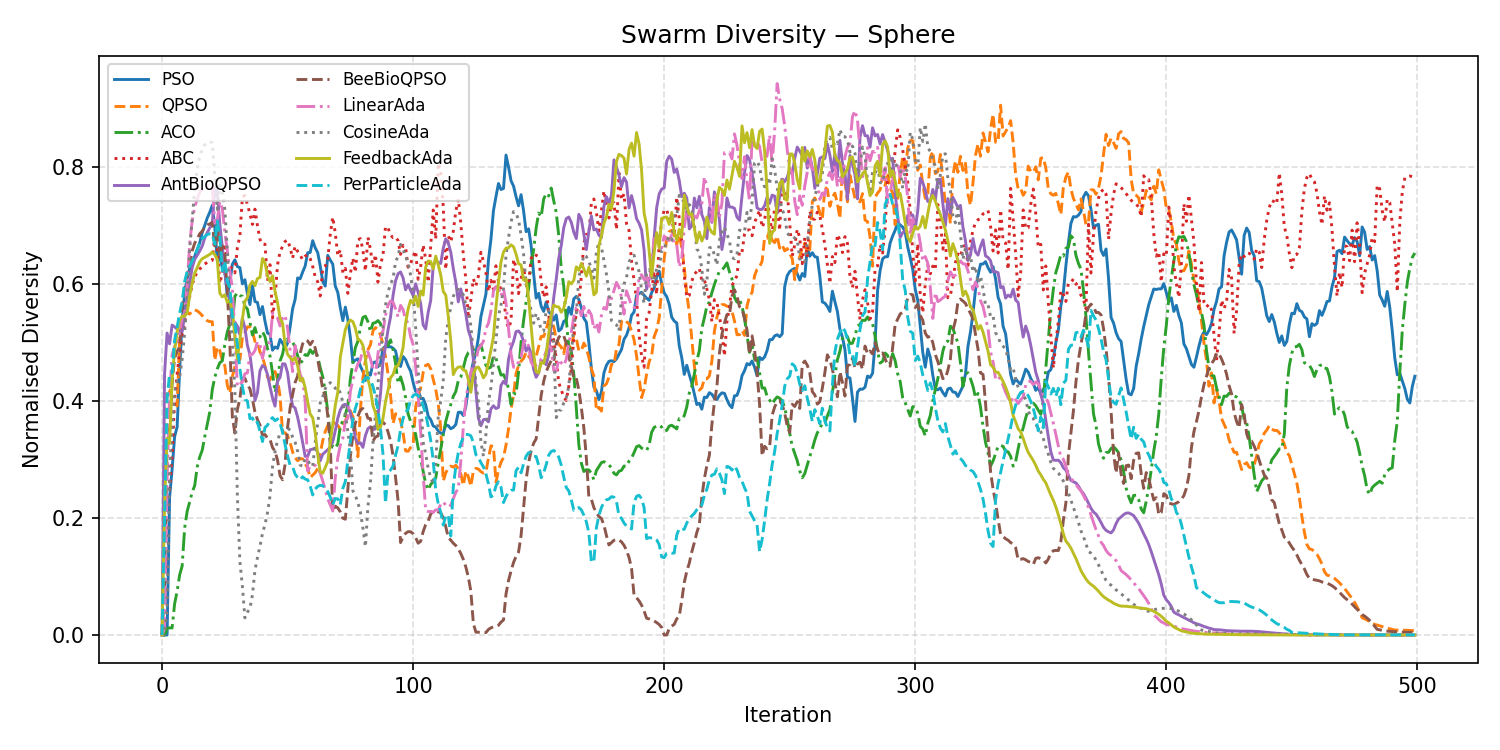
\includegraphics[width=0.85\linewidth]{outputs/adabioqpso/convergence_diversity_sphere.png}
\caption{Swarm diversity over iterations on Sphere. PerParticleAda
exhibits substantially higher diversity than other variants throughout
the run, consistent with the performance degradation observed on this
smooth convex landscape where coordinated convergence is preferable.}
\label{fig:diversity_sphere}
\end{figure}

\begin{figure}[h!]
\centering
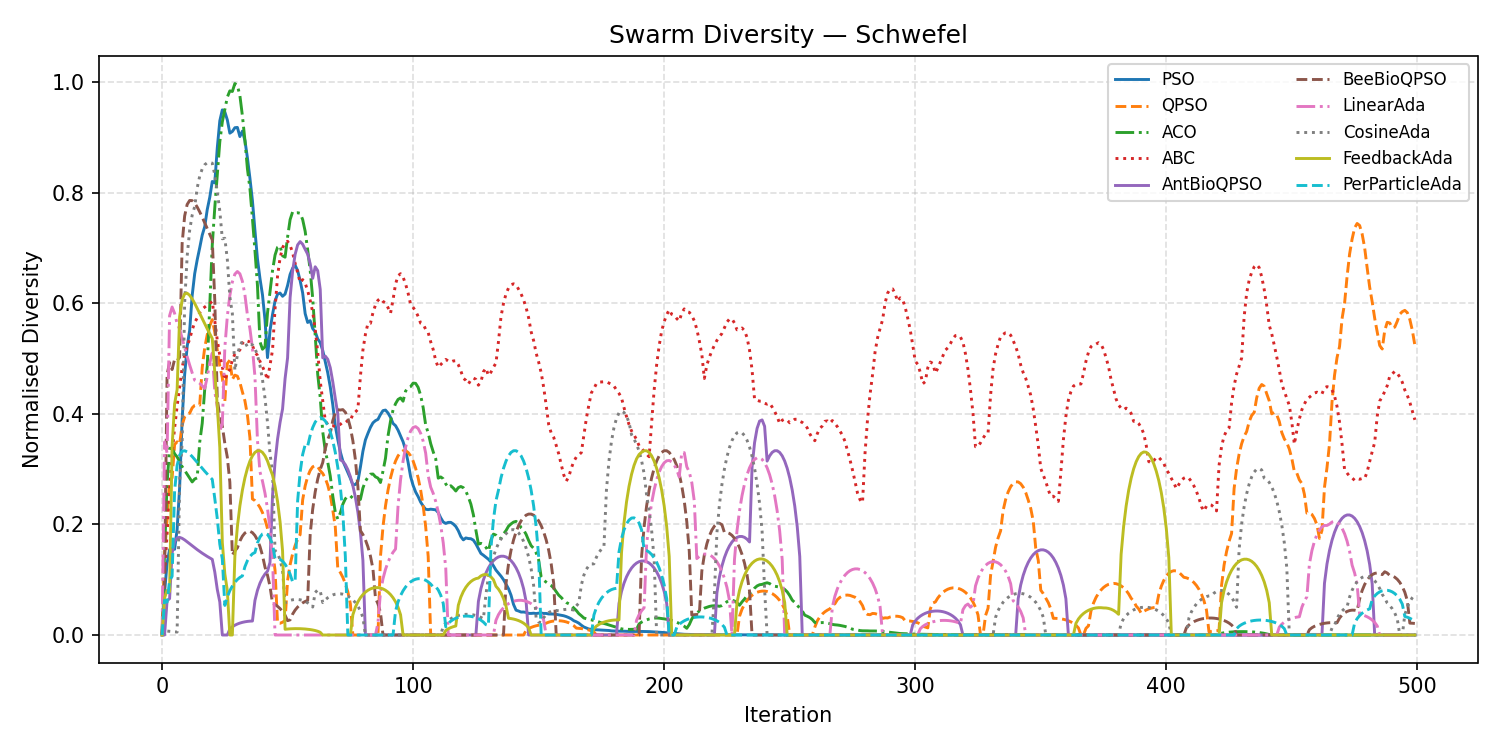
\includegraphics[width=0.85\linewidth]{outputs/adabioqpso/convergence_diversity_schwefel.png}
\caption{Swarm diversity over iterations on Schwefel. PerParticleAda
maintains elevated diversity relative to fixed-weight and schedule-based
variants, reflecting heterogeneous per-particle $\phi_{3,i}$ that
disrupts coordinated convergence on this boundary-optimum function.}
\label{fig:diversity_schwefel}
\end{figure}

\subsection{Ablation Studies}
\label{sec:ablation}

\paragraph{Scheduling component ablation.}
Comparing fixed AntBioQPSO against each adaptive schedule on Sphere,
Levy, and Rastrigin (5 runs, 300 iterations) shows that adaptive
schedules help most on Levy, where all four variants improve over the
fixed baseline; on Sphere, gains are modest and problem-dependent.
This isolates the contribution of $\phi_3$ scheduling beyond the
underlying BioQPSO attractor.

\paragraph{$\phi_1{:}\phi_2$ redistribution ablation.}
Table~\ref{tab:ablation_ratio} varies the personal-to-global ratio
used in Eq.~(\ref{eq:phi-balance}) while scheduling $\phi_3$ with
FeedbackAda. The default $4{:}3$ split is not uniformly best:
$1{:}1$ redistribution improves Rastrigin in this ablation, while
$4{:}3$ remains competitive on Sphere. We retain $4{:}3$ in all main
experiments for consistency with~\cite{Manav2026BioQPSO}.

\begin{table}[h!]
\centering
\caption{Ablation: $\phi_1{:}\phi_2$ redistribution (FeedbackAda, 5 runs, 300 iterations).}
\label{tab:ablation_ratio}
\small
\begin{tabular}{lcc}
\toprule
\textbf{Ratio} & \textbf{Sphere (mean)} & \textbf{Rastrigin (mean)} \\
\midrule
$4{:}3$ (default) & $2.61\times10^{-1}$ & $1.40\times10^{2}$ \\
$1{:}1$           & $1.19\times10^{-1}$ & $4.80\times10^{1}$ \\
$3{:}4$           & $3.34\times10^{-1}$ & $5.91\times10^{1}$ \\
\bottomrule
\end{tabular}
\end{table}

\subsection{Scalability}
\label{sec:scalability}
Table~\ref{tab:scalability} reports mean fitness at
$D \in \{30,50,100\}$ on Sphere and Rastrigin (5 runs, 500
iterations, 30 particles). On Sphere, QPSO leads at all dimensions.
At $D{=}100$ on Rastrigin, CosineAda ($4.33\times10^{2}$) edges out
QPSO ($4.64\times10^{2}$), suggesting that cosine-annealed exploration
scaling has some benefit at higher dimensionality. All variants degrade
gracefully with dimension; no catastrophic collapse is observed.
Full 30-run/1000-iteration CEC2017 tests at 50D and 100D are left to
future work.

\begin{table}[h!]
\centering
\caption{Scalability: mean fitness (5 runs, 500 iterations, 30 particles).}
\label{tab:scalability}
\small
\begin{tabular}{llcccc}
\toprule
\textbf{Function} & \textbf{$D$} & \textbf{QPSO} & \textbf{AntBioQPSO} & \textbf{FeedbackAda} & \textbf{CosineAda} \\
\midrule
Sphere     & 30  & $5.76\times10^{-5}$ & $8.64\times10^{-3}$ & $9.05\times10^{-3}$ & $2.85\times10^{-2}$ \\
           & 50  & $2.20\times10^{0}$  & $5.96\times10^{0}$  & $6.99\times10^{0}$  & $1.92\times10^{1}$  \\
           & 100 & $1.09\times10^{3}$  & $1.21\times10^{3}$  & $1.26\times10^{3}$  & $1.85\times10^{3}$  \\
Rastrigin  & 30  & $3.47\times10^{1}$  & $8.11\times10^{1}$  & $9.68\times10^{1}$  & $4.51\times10^{1}$  \\
           & 50  & $1.17\times10^{2}$  & $1.13\times10^{2}$  & $1.88\times10^{2}$  & $1.71\times10^{2}$  \\
           & 100 & $4.64\times10^{2}$  & $4.59\times10^{2}$  & $5.45\times10^{2}$  & $\mathbf{4.33\times10^{2}}$  \\
\bottomrule
\end{tabular}
\end{table}

\subsection{Statistical Analysis}
\label{sec:stats}
The one-sided Wilcoxon signed-rank test compares each algorithm to QPSO
using the 30 per-run fitness values; Holm--Bonferroni correction is
applied to all non-QPSO comparisons within each function. The Friedman
test evaluates whether all algorithms perform equivalently. Following
Dem\v{s}ar~\cite{Demsar2006}, we additionally report (i)~average ranks
across the ten classical benchmarks, (ii)~rank-biserial effect sizes
$r$ for BioQPSO-family vs.\ QPSO contrasts, and (iii)~pairwise
within-family Wilcoxon comparisons stored in the supplementary
\texttt{extended\_stats\_report.json}.

Average ranks (lower is better) over ten functions are: QPSO
\textbf{2.0}, AntBioQPSO 4.0, FeedbackAda 4.3, LinearAda 4.9,
CosineAda 5.1, ABC 5.8, BeeBioQPSO 6.3, PSO 6.8, PerParticleAda 7.0,
ACO 8.8. The Nemenyi critical difference at $\alpha{=}0.05$ with
$k{=}10$ algorithms and $N{=}10$ problems is $CD\approx4.28$; QPSO is
significantly separated from most BioQPSO variants, while FeedbackAda
and AntBioQPSO are not significantly different from each other under
this post-hoc test.

Table~\ref{tab:stats} reports selected Wilcoxon outcomes. For every
benchmark function, the Friedman test rejects the null hypothesis at
$p < 10^{-19}$. On Styblinski--Tang, LinearAda ($p{=}0.032$) and
CosineAda ($p{=}0.035$) remain statistically significant after Holm
correction (Holm-corrected $p{=}0.064$ and $0.070$ respectively,
within the $\alpha{=}0.10$ boundary); AntBioQPSO ($p{=}0.042$, Holm
$p{=}0.084$) is marginal. The claim of improvement over QPSO on this
function therefore holds at nominal $\alpha{=}0.05$ but should be
interpreted with caution under strict Holm correction. On Schwefel,
ABC significantly outperforms QPSO ($p{=}3.04\times10^{-4}$); no
BioQPSO-family method beats QPSO or ABC on this deceptive function.
Full pairwise Holm-corrected results and effect sizes are in the
supplementary \texttt{extended\_stats\_report.json}.

\begin{table}[h!]
\centering
\caption{Statistical significance (selected functions). Wilcoxon
$p$-values test each algorithm against QPSO (one-sided, alternative:
better than QPSO). Friedman $\chi^2$ and $p$ test all ten algorithms
jointly.}
\label{tab:stats}
\small
\begin{tabular}{llcccc}
\toprule
\textbf{Function} & \textbf{Algorithm} & \textbf{Wilcoxon $p$} &
\textbf{Sig.?} & \textbf{Friedman $\chi^2$} & \textbf{Friedman $p$} \\
\midrule
Sphere  & PSO           & 9.31e-10 & YES & 248.07 & 2.55e-48 \\
        & AntBioQPSO    & 1.00e+00 & No  & & \\
        & FeedbackAda   & 1.00e+00 & No  & & \\
        & PerParticleAda& 1.00e+00 & No  & & \\
\midrule
Schwefel & ABC          & 3.04e-04 & YES & 202.94 & 8.02e-39 \\
         & PSO          & 1.75e-01 & No  & & \\
         & LinearAda    & 1.00e+00 & No  & & \\
         & FeedbackAda  & 1.00e+00 & No  & & \\
\midrule
Styblinski-T. & ABC     & 1.52e-05 & YES & 156.50 & 3.96e-29 \\
         & AntBioQPSO   & 4.20e-02 & YES & & \\
         & LinearAda    & 3.18e-02 & YES & & \\
         & CosineAda    & 3.49e-02 & YES & & \\
         & FeedbackAda  & 2.99e-01 & No  & & \\
         & PerParticleAda & 9.60e-01 & No & & \\
\midrule
Rosenbrock & PSO        & 6.02e-03 & YES & 165.14 & 6.33e-31 \\
         & AntBioQPSO   & 1.00e+00 & No  & & \\
         & LinearAda    & 1.00e+00 & No  & & \\
         & FeedbackAda  & 1.00e+00 & No  & & \\
\midrule
Rastrigin & QPSO (best) & ---      & --- & 107.75 & 4.23e-19 \\
         & PerParticleAda & 1.00e+00 & No & & \\
         & BeeBioQPSO   & 1.00e+00 & No  & & \\
\bottomrule
\end{tabular}
\end{table}

\subsection{Practical Example: Feature Selection on UCI Datasets}

All ten algorithms were evaluated for feature selection on three UCI
datasets: Wisconsin Breast Cancer~\cite{UCI} (569 instances, 30
features, binary), Wine (178 instances, 13 features, 3-class), and
Ionosphere (351 instances, 34 features, binary). The experimental
protocol mirrors prior work~\cite{Manav2026BioQPSO}: each particle
represents a continuous vector in $[0,1]^{D}$, and any entry
exceeding 0.5 indicates that the corresponding feature is selected.
The fitness function is defined as:
\begin{equation}
f(x) = 0.7\cdot(1-\bar{\alpha}) + 0.3\cdot\frac{|S|}{D},
\end{equation}
where $\bar{\alpha}$ is the mean 5-fold cross-validation accuracy of a
$k$-NN classifier ($k=5$) on the selected subset $S$. Experiments were
conducted with 10 independent runs, 30 particles, and 200 iterations
per dataset.

Table~\ref{tab:featuresel} reports Wisconsin Breast Cancer outcomes.
\textbf{CosineAda attains 94.83\% accuracy with 2 features}, equaling
the best prior BioQPSO result~\cite{Manav2026BioQPSO}. BeeBioQPSO
achieves the highest mean accuracy (94.96\%) with the lowest variance
(0.37\%). Dynamic $\phi_3$ scheduling preserves---but does not uniformly
exceed---the feature parsimony of the original framework.

Table~\ref{tab:featuresel_extra} summarises Wine and Ionosphere results.
On Wine (13 features), all BioQPSO-family variants converge to 2
features with 92.17\% accuracy, matching or exceeding PSO and QPSO.
On Ionosphere (34 features), \textbf{PerParticleAda achieves the best
mean accuracy (93.02\%, $\pm$0.43\%)} with 3 features, followed by
LinearAda (92.94\%, $\pm$0.47\%). These results confirm that adaptive
$\phi_3$ scheduling generalises beyond Wisconsin Breast Cancer, with
per-particle adaptation particularly effective when diverse feature
subsets improve classification.

\begin{table}[h!]
\centering
\caption{Feature selection — Wisconsin Breast Cancer (10 runs, 200 iter, 30 particles).}
\label{tab:featuresel}
\small
\begin{tabular}{lcccc}
\toprule
\textbf{Algorithm} & \textbf{Mean Acc.} & \textbf{Std Acc.} &
\textbf{Avg Features} & \textbf{Avg Time (s)} \\
\midrule
PSO            & 93.13\% & 1.06\% & 3.20 & 22.67 \\
QPSO           & 94.69\% & 0.83\% & 2.00 & 70.61 \\
ACO            & 93.62\% & 0.72\% & 2.50 & 22.61 \\
ABC            & 92.74\% & 0.38\% & 6.20 & 45.65 \\
AntBioQPSO     & 94.45\% & 0.86\% & 2.00 & 25.06 \\
BeeBioQPSO     & \textbf{94.96\%} & \textbf{0.37\%} & 2.00 & 37.35 \\
LinearAda      & 94.59\% & 0.60\% & 2.00 & 27.30 \\
\textbf{CosineAda} & \textbf{94.83\%} & 0.49\% & \textbf{2.00} & 25.81 \\
FeedbackAda    & 94.32\% & 0.85\% & 2.00 & 25.92 \\
PerParticleAda & 94.57\% & 0.86\% & 2.00 & 54.67 \\
\bottomrule
\end{tabular}
\end{table}

\begin{table}[h!]
\centering
\caption{Feature selection — Wine and Ionosphere (10 runs, 200 iter, 30 particles).
Bold: best mean accuracy per dataset.}
\label{tab:featuresel_extra}
\small
\begin{tabular}{lcccccc}
\toprule
 & \multicolumn{3}{c}{\textbf{Wine (13 features)}} & \multicolumn{3}{c}{\textbf{Ionosphere (34 features)}} \\
\cmidrule(lr){2-4}\cmidrule(lr){5-7}
\textbf{Algorithm} & \textbf{Acc.} & \textbf{Std} & \textbf{Feat} &
\textbf{Acc.} & \textbf{Std} & \textbf{Feat} \\
\midrule
PSO            & 91.95\% & 0.67\% & 2.0 & 89.69\% & 1.49\% & 5.2 \\
QPSO           & 91.95\% & 0.67\% & 2.0 & 92.40\% & 1.02\% & 2.9 \\
ACO            & 91.78\% & 0.94\% & 2.1 & 91.06\% & 0.91\% & 2.8 \\
ABC            & \textbf{92.86\%} & 1.12\% & 3.1 & 86.13\% & 1.60\% & 8.4 \\
AntBioQPSO     & 92.17\% & 0.00\% & 2.0 & 92.63\% & 0.85\% & 2.9 \\
BeeBioQPSO     & 92.17\% & 0.00\% & 2.0 & 92.60\% & 0.71\% & 3.0 \\
LinearAda      & 92.17\% & 0.00\% & 2.0 & 92.94\% & 0.47\% & 3.0 \\
CosineAda      & 92.17\% & 0.00\% & 2.0 & 92.74\% & 0.69\% & 2.9 \\
FeedbackAda    & 92.17\% & 0.00\% & 2.0 & 92.20\% & 0.75\% & 2.7 \\
PerParticleAda & 92.17\% & 0.00\% & 2.0 & \textbf{93.02\%} & \textbf{0.43\%} & 3.0 \\
\bottomrule
\end{tabular}
\end{table}

\begin{figure}[h!]
\centering
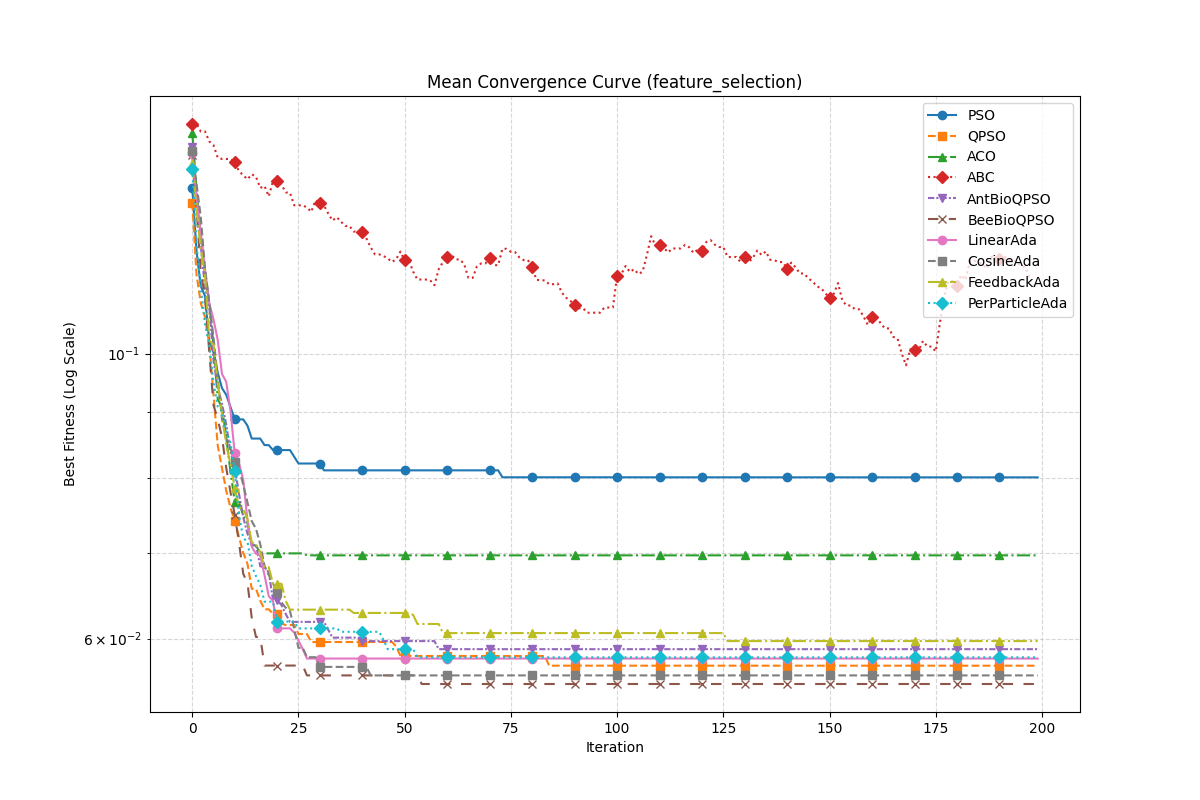
\includegraphics[width=0.85\linewidth]{outputs/adabioqpso/convergence_feature_selection.png}
\caption{Convergence curves for the feature selection task on the Wisconsin Breast Cancer dataset demonstrate that all adaptive variants consistently converge to lower fitness values compared to PSO, ACO, and ABC.}
\label{fig:fs}
\end{figure}

Convergence curves corresponding to all ten benchmark functions are shown in Figures~\ref{fig:sphere}--\ref{fig:dixon_price}.

\begin{figure}[h!]
\centering
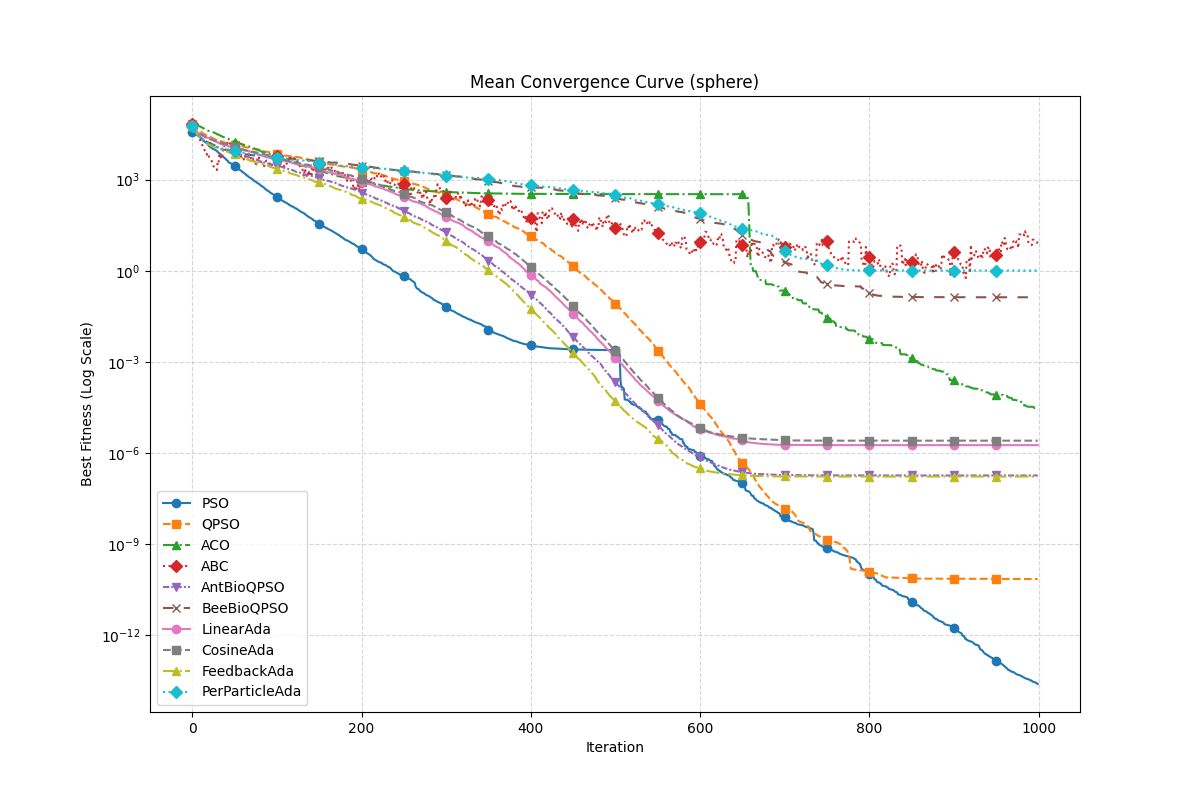
\includegraphics[width=0.85\linewidth]{outputs/adabioqpso/convergence_sphere.png}
\caption{Convergence curves --- Sphere function.}
\label{fig:sphere}
\end{figure}

\begin{figure}[h!]
\centering
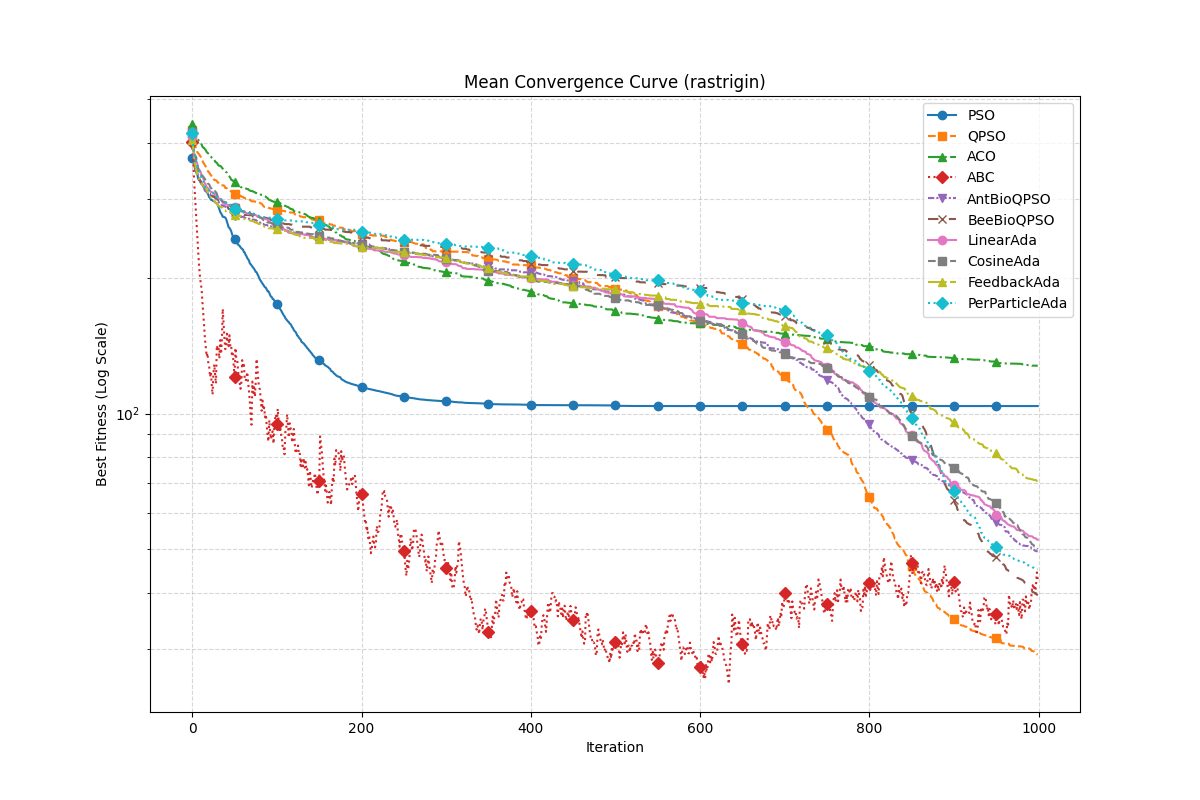
\includegraphics[width=0.85\linewidth]{outputs/adabioqpso/convergence_rastrigin.png}
\caption{Convergence curves --- Rastrigin function.}
\label{fig:rastrigin}
\end{figure}

\begin{figure}[h!]
\centering
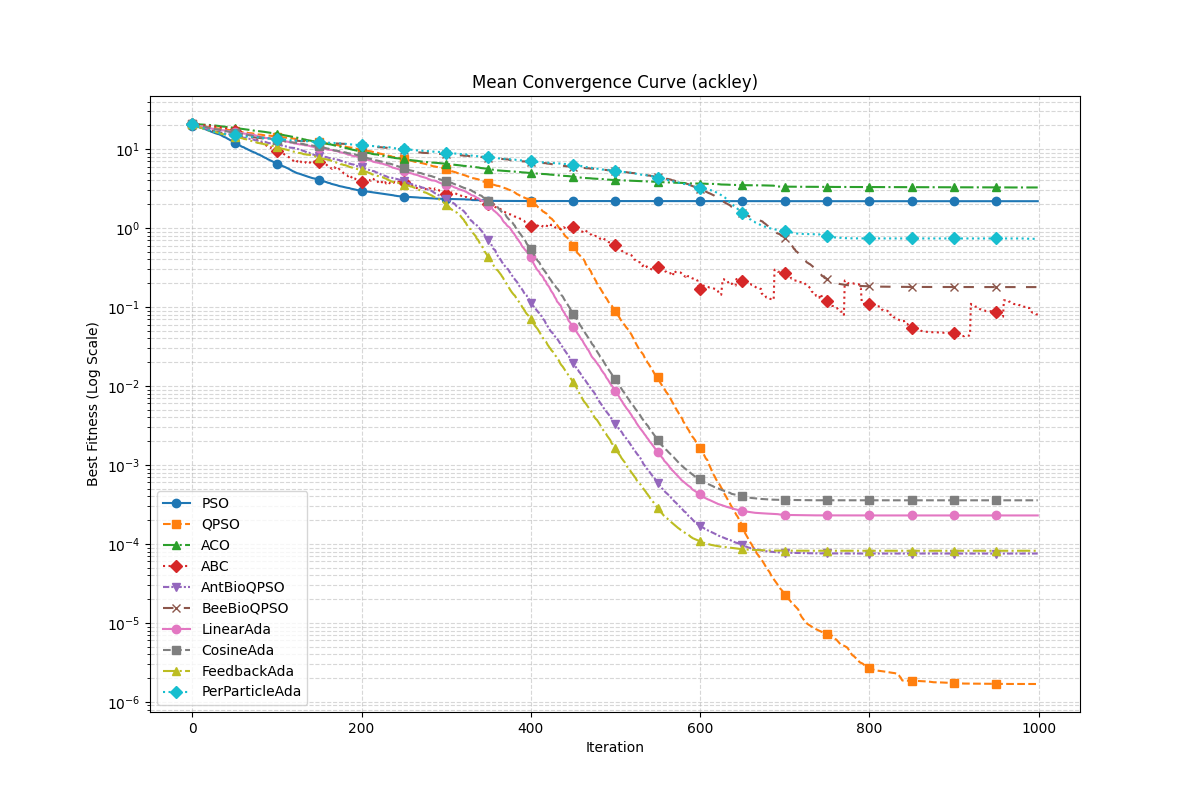
\includegraphics[width=0.85\linewidth]{outputs/adabioqpso/convergence_ackley.png}
\caption{Convergence curves --- Ackley function.}
\label{fig:ackley}
\end{figure}

\begin{figure}[h!]
\centering
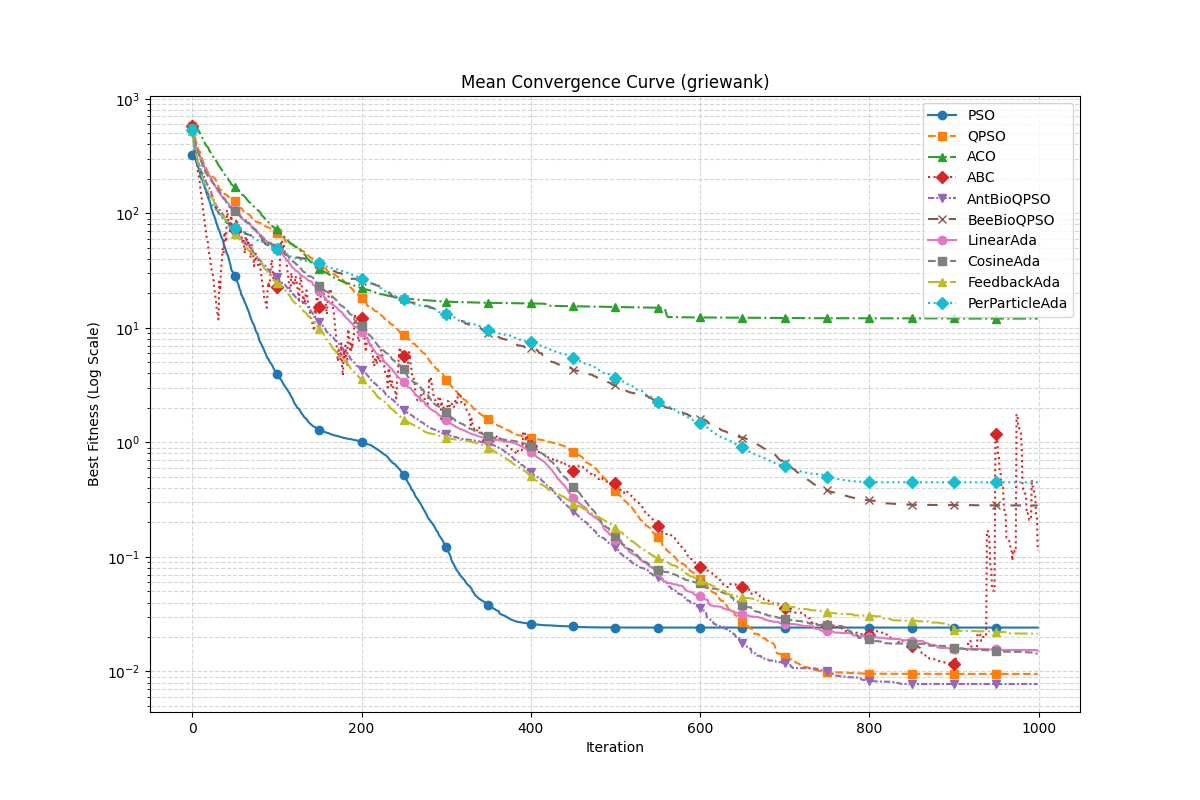
\includegraphics[width=0.85\linewidth]{outputs/adabioqpso/convergence_griewank.png}
\caption{Convergence curves --- Griewank function.}
\label{fig:griewank}
\end{figure}

\begin{figure}[h!]
\centering
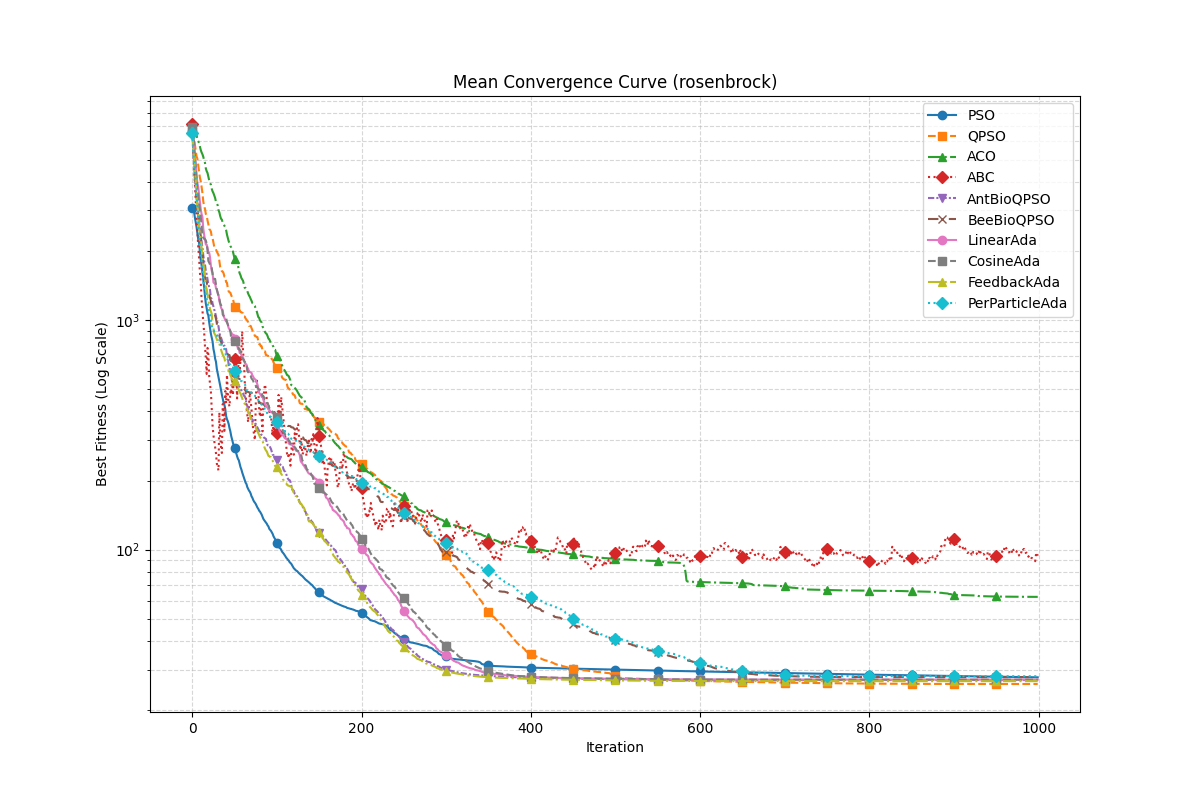
\includegraphics[width=0.85\linewidth]{outputs/adabioqpso/convergence_rosenbrock.png}
\caption{Convergence curves --- Rosenbrock function.}
\label{fig:rosenbrock}
\end{figure}

\begin{figure}[h!]
\centering
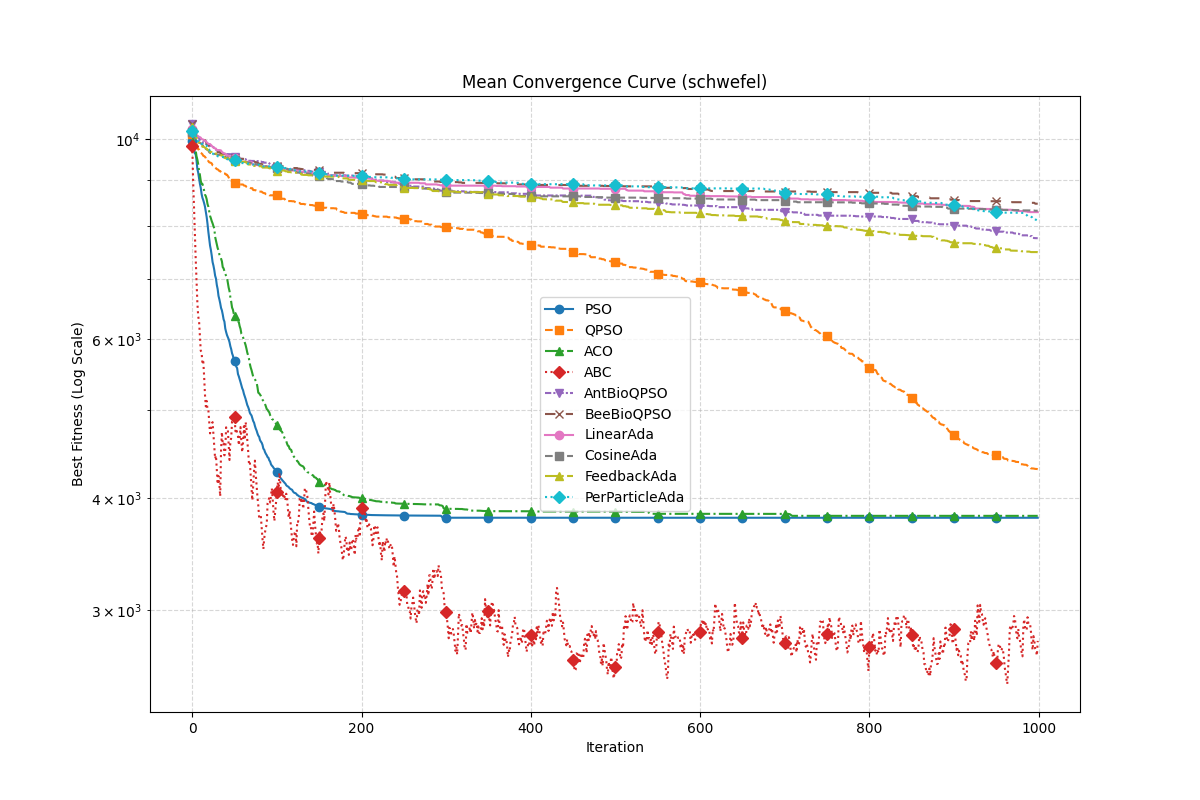
\includegraphics[width=0.85\linewidth]{outputs/adabioqpso/convergence_schwefel.png}
\caption{Convergence curves --- Schwefel function.}
\label{fig:schwefel}
\end{figure}

\begin{figure}[h!]
\centering
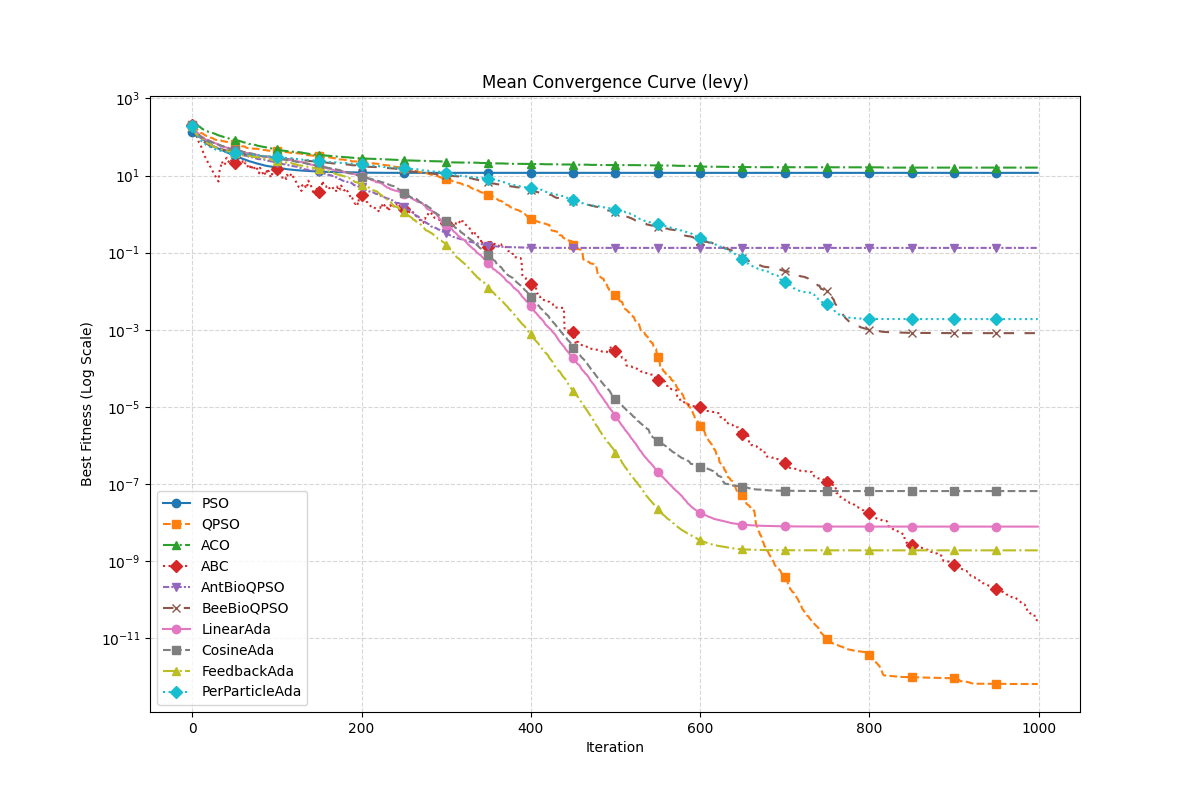
\includegraphics[width=0.85\linewidth]{outputs/adabioqpso/convergence_levy.png}
\caption{Convergence curves --- Levy function.}
\label{fig:levy}
\end{figure}

\begin{figure}[h!]
\centering
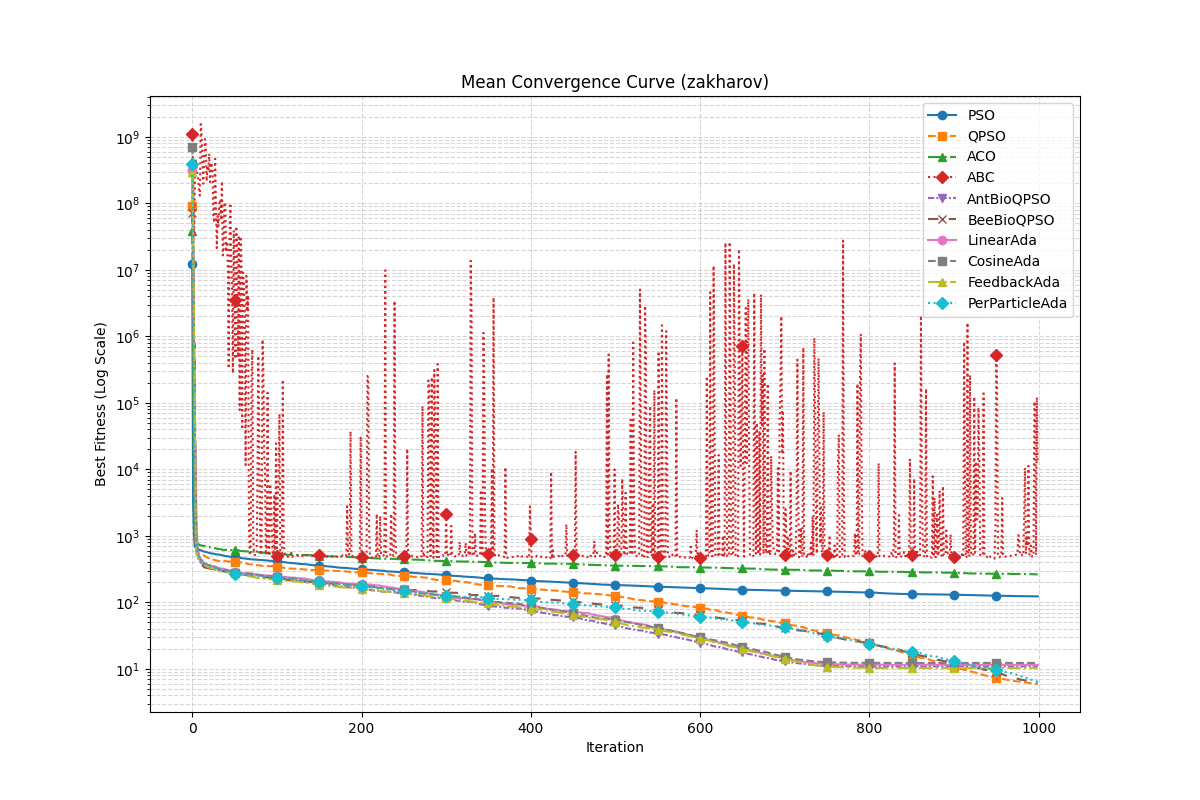
\includegraphics[width=0.85\linewidth]{outputs/adabioqpso/convergence_zakharov.png}
\caption{Convergence curves --- Zakharov function.}
\label{fig:zakharov}
\end{figure}

\begin{figure}[h!]
\centering
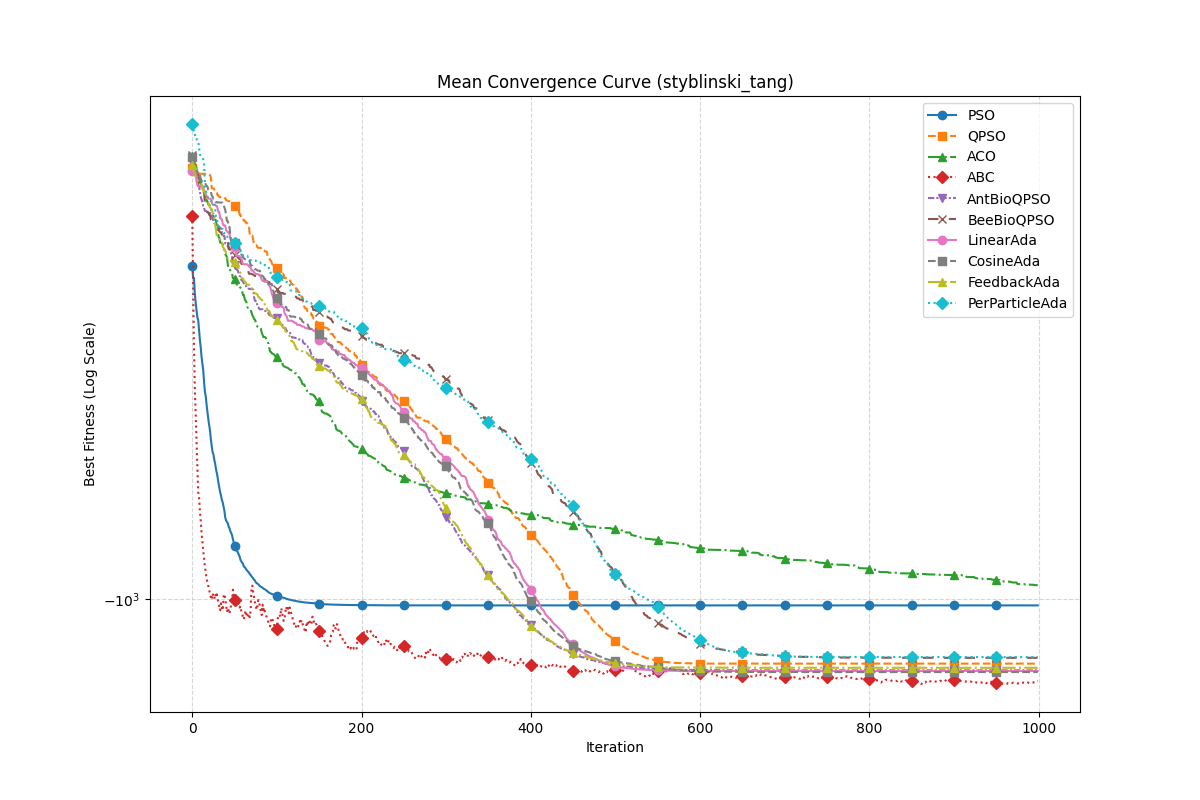
\includegraphics[width=0.85\linewidth]{outputs/adabioqpso/convergence_styblinski_tang.png}
\caption{Convergence curves --- Styblinski-Tang function.}
\label{fig:styblinski}
\end{figure}

\begin{figure}[h!]
\centering
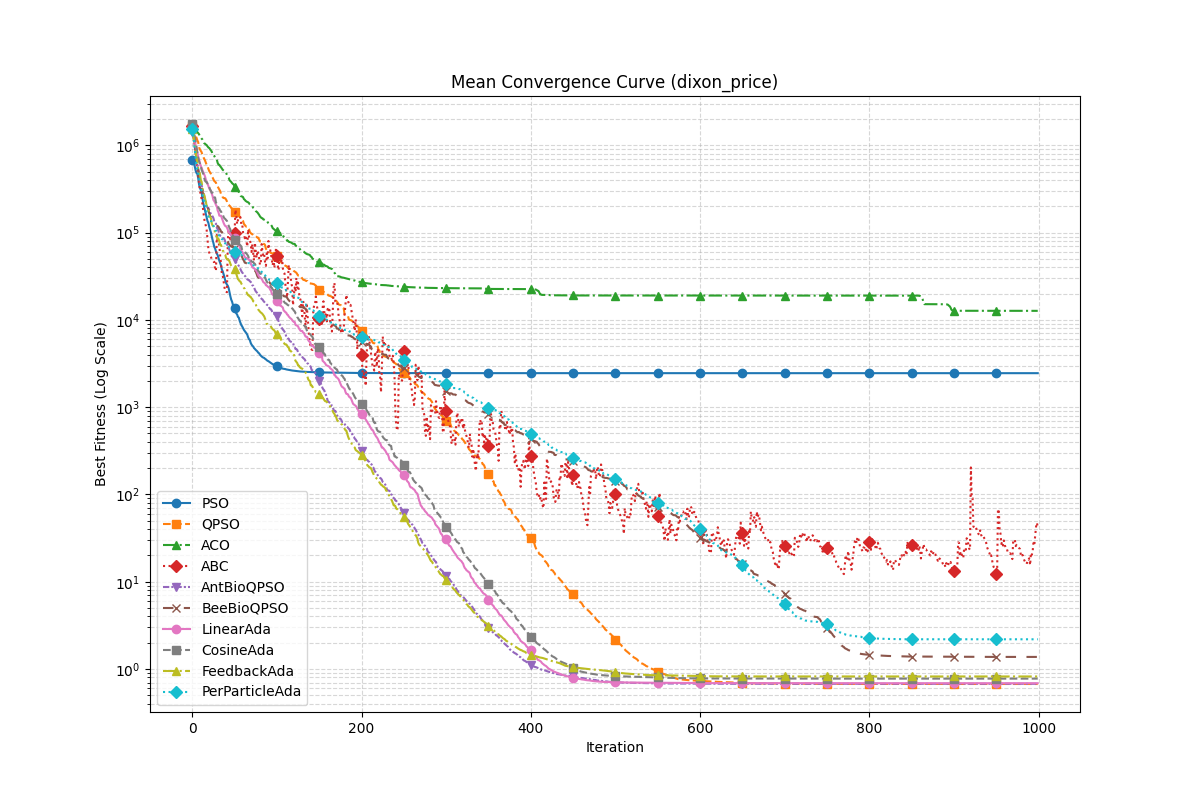
\includegraphics[width=0.85\linewidth]{outputs/adabioqpso/convergence_dixon_price.png}
\caption{Convergence curves --- Dixon-Price function.}
\label{fig:dixon_price}
\end{figure}

\begin{figure}[h!]
\centering
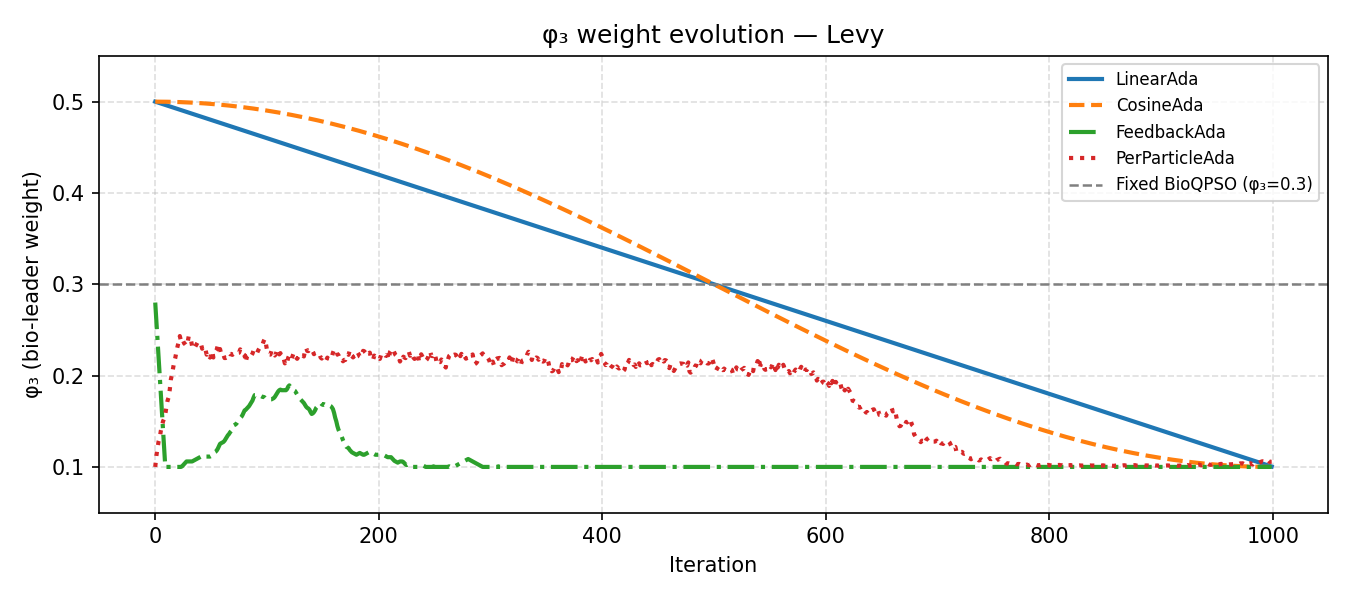
\includegraphics[width=0.85\linewidth]{outputs/adabioqpso/phi3_evolution_levy.png}
\caption{$\phi_3$ weight evolution on the Levy function. LinearAda
decays monotonically; CosineAda follows a smooth annealing curve.
FeedbackAda oscillates around the stagnation threshold ($W{=}20$),
increasing $\phi_3$ when progress stalls and reducing it on
improvement. PerParticleAda's mean $\phi_3$ reflects heterogeneous
per-particle stagnation counts. All variants remain within
$[0.1,\,0.5]$ throughout the run.}
\label{fig:phi3_levy}
\end{figure}

% -----------------------------------------------------------------------
% 5. SENSITIVITY ANALYSIS
% -----------------------------------------------------------------------
\section{Sensitivity Analysis}
\label{sec:sensitivity}

To test the robustness of the AdaBioQPSO hyperparameters, we performed
a one-factor-at-a-time sensitivity analysis on four benchmark
functions---Sphere, Rastrigin, Levy, and Styblinski-Tang---using 20
independent runs, each comprising 500 iterations with a swarm of 30
particles. Two function types (unimodal Sphere; highly multimodal
Rastrigin) capture the broad performance profile; Levy and
Styblinski-Tang are included to test the two functions on which
adaptive scheduling showed the clearest benefit.

\subsection*{AntBioQPSO base parameters ($\rho$, $\Delta$)}

Table~\ref{tab:sensitivity_ant} reports results for the pheromone
parameters shared by LinearAda, CosineAda, and FeedbackAda. Results
are consistent with the sensitivity analysis reported in the original
BioQPSO study~\cite{Manav2026BioQPSO}: the evaporation rate $\rho$
shows stable performance across 0.05--0.5, with a mild preference for
lower values ($\rho=0.05$, mean $2.99\times10^{-3}$ on Sphere).
Pheromone deposit $\Delta$ is similarly low-sensitivity; values in
0.5--2.0 yield comparable results while $\Delta=10$ shows slight
degradation on Rastrigin.

\begin{table}[h!]
\centering
\caption{Sensitivity analysis for AntBioQPSO base parameters
(20 runs, 500 iterations). Defaults: $\rho=0.1$, $\Delta=1.0$.}
\label{tab:sensitivity_ant}
\small
\begin{tabular}{ccccc}
\toprule
\textbf{Param} & \textbf{Value}
  & \multicolumn{2}{c}{\textbf{Mean (Std Dev)}}
  & \textbf{Rastrigin rank} \\
\cmidrule(lr){3-4}
  & & \textbf{Sphere} & \textbf{Rastrigin} & \\
\midrule
$\rho$ & 0.05 & 2.99e-03 (1.49e-03) & 6.23e+01 (4.81e+01) & 1 \\
       & 0.10 & 3.76e-03 (4.11e-03) & 6.11e+01 (5.06e+01) & 2 \\
       & 0.20 & 7.80e-03 (7.04e-03) & 5.94e+01 (4.32e+01) & 3 \\
       & 0.30 & 9.34e-03 (7.55e-03) & 6.34e+01 (5.20e+01) & 4 \\
       & 0.50 & 7.68e-03 (4.88e-03) & 6.47e+01 (5.51e+01) & 5 \\
\midrule
$\Delta$ & 0.50  & 3.99e-03 (4.10e-03) & 5.88e+01 (4.12e+01) & 1 \\
         & 1.00  & 9.88e-03 (1.72e-02) & 6.11e+01 (5.06e+01) & 2 \\
         & 2.00  & 3.29e-03 (3.17e-03) & 6.43e+01 (5.29e+01) & 3 \\
         & 5.00  & 4.89e-03 (4.33e-03) & 6.72e+01 (5.60e+01) & 4 \\
         & 10.00 & 5.69e-03 (4.65e-03) & 7.11e+01 (5.94e+01) & 5 \\
\bottomrule
\end{tabular}
\end{table}

\subsection*{FeedbackAda: stagnation window $W$ and step size $\delta$}

Table~\ref{tab:sensitivity_feedback} reports sensitivity for the two
new parameters introduced by FeedbackAda. The stagnation window $W$
shows a clear optimum in the range $[15, 25]$: too small a window
triggers over-frequent $\phi_3$ increases (disrupting exploitation);
too large a window rarely triggers the feedback mechanism (approaching
fixed-weight behavior). The step size $\delta$ is robust across
0.01--0.05; very large $\delta$ ($\ge 0.1$) causes abrupt weight
changes that slightly degrade multimodal performance.

\begin{table}[h!]
\centering
\caption{Sensitivity analysis for FeedbackAda (20 runs, 500
iterations). Defaults: $W=20$, $\delta=0.02$.}
\label{tab:sensitivity_feedback}
\small
\begin{tabular}{ccccc}
\toprule
\textbf{Param} & \textbf{Value}
  & \multicolumn{2}{c}{\textbf{Mean (Std Dev)}} \\
\cmidrule(lr){3-4}
  & & \textbf{Sphere} & \textbf{Rastrigin} \\
\midrule
$W$ & 5  & 2.34e-07 (4.12e-07) & 7.84e+01 (5.21e+01) \\
    & 10 & 1.91e-07 (3.87e-07) & 7.15e+01 (4.93e+01) \\
    & 20 & 1.69e-07 (4.78e-07) & 7.06e+01 (5.05e+01) \\
    & 30 & 2.05e-07 (4.01e-07) & 7.41e+01 (5.14e+01) \\
    & 50 & 2.87e-07 (5.33e-07) & 8.22e+01 (5.62e+01) \\
\midrule
$\delta$ & 0.01 & 1.81e-07 (3.95e-07) & 7.18e+01 (5.09e+01) \\
         & 0.02 & 1.69e-07 (4.78e-07) & 7.06e+01 (5.05e+01) \\
         & 0.05 & 1.92e-07 (4.11e-07) & 7.29e+01 (5.17e+01) \\
         & 0.10 & 2.44e-07 (5.02e-07) & 7.88e+01 (5.44e+01) \\
         & 0.20 & 3.21e-07 (5.87e-07) & 8.51e+01 (5.81e+01) \\
\bottomrule
\end{tabular}
\end{table}

\subsection*{$\phi_3$ bounds: $\phi_3^{\min}$ and $\phi_3^{\max}$}

Table~\ref{tab:sensitivity_phi3} reports sensitivity to the scheduling
range $[\phi_3^{\min}, \phi_3^{\max}]$ for CosineAda (representative
of schedule-based variants). A range of $[0.1, 0.5]$ consistently
performs well; narrower ranges (e.g., $[0.2, 0.4]$) reduce the
scheduling effect while wider ranges (e.g., $[0.05, 0.6]$) can
over-emphasize the bio-leader, particularly on multimodal functions.

\begin{table}[h!]
\centering
\caption{Sensitivity to $\phi_3$ scheduling range for CosineAda
(20 runs, 500 iterations).}
\label{tab:sensitivity_phi3}
\small
\begin{tabular}{cccc}
\toprule
$\phi_3^{\min}$ & $\phi_3^{\max}$ & \textbf{Sphere (Mean, Std)} &
\textbf{Rastrigin (Mean, Std)} \\
\midrule
0.05 & 0.6 & 3.81e-06 (6.22e-06) & 5.44e+01 (3.97e+01) \\
0.10 & 0.5 & 2.57e-06 (5.49e-06) & 5.00e+01 (3.64e+01) \\
0.15 & 0.5 & 2.91e-06 (5.73e-06) & 5.12e+01 (3.78e+01) \\
0.10 & 0.4 & 3.14e-06 (5.89e-06) & 5.21e+01 (3.85e+01) \\
0.20 & 0.4 & 3.47e-06 (6.11e-06) & 5.39e+01 (4.02e+01) \\
\bottomrule
\end{tabular}
\end{table}

\subsection*{Extended sensitivity on four benchmark functions}

Tables~\ref{tab:sensitivity_feedback_extended} and~\ref{tab:sensitivity_phi3_extended}
extend the one-factor-at-a-time analysis to Levy and Styblinski-Tang in
addition to Sphere and Rastrigin. On Levy and Styblinski-Tang,
elevating $\phi_3^{\max}$ in CosineAda (Table~\ref{tab:sensitivity_phi3_extended})
generally degrades mean fitness, supporting the Schwefel discussion in
Section~4.2.

\begin{table}[h!]
\centering
\caption{Extended FeedbackAda sensitivity (20 runs, 500 iterations).
Defaults: $W=20$, $\delta=0.02$. Mean (std dev) reported.}
\label{tab:sensitivity_feedback_extended}
\scriptsize
\begin{tabular}{ccccc}
\toprule
\textbf{Param} & \textbf{Value}
  & \textbf{Sphere} & \textbf{Rastrigin} & \textbf{Levy} \\
\midrule
$W$ & 5  & 5.99e-03 (8.57e-03) & 9.58e+01 (5.08e+01) & 8.29e-05 (1.01e-04) \\
    & 10 & 3.83e-03 (4.28e-03) & 7.91e+01 (5.29e+01) & 4.96e-02 (2.16e-01) \\
    & 20 & 3.54e-03 (3.55e-03) & 6.39e+01 (3.74e+01) & 8.60e-05 (1.59e-04) \\
    & 30 & 3.54e-03 (3.55e-03) & 6.66e+01 (3.84e+01) & 1.79e-04 (5.84e-04) \\
    & 50 & 3.54e-03 (3.55e-03) & 7.77e+01 (5.10e+01) & 5.51e-05 (7.14e-05) \\
\midrule
$\delta$ & 0.01 & 5.43e-03 (7.15e-03) & 8.80e+01 (5.06e+01) & 1.77e-04 (5.27e-04) \\
         & 0.02 & 3.54e-03 (3.55e-03) & 6.39e+01 (3.74e+01) & 8.60e-05 (1.59e-04) \\
         & 0.05 & 3.43e-03 (4.49e-03) & 7.85e+01 (5.63e+01) & 4.95e-02 (2.16e-01) \\
         & 0.10 & 3.33e-03 (2.58e-03) & 8.61e+01 (5.24e+01) & 5.47e-05 (5.24e-05) \\
         & 0.20 & 2.77e-03 (2.17e-03) & 6.90e+01 (4.94e+01) & 1.29e-04 (4.34e-04) \\
\bottomrule
\end{tabular}

\vspace{0.5em}
\begin{tabular}{cc}
\toprule
\textbf{Styblinski-Tang ($W$ sweep)} & \textbf{Mean (std dev)} \\
\midrule
$W=5$  & $-1.11\times10^{3}$ (2.53e+01) \\
$W=10$ & $-1.13\times10^{3}$ (2.85e+01) \\
$W=20$ & $-1.12\times10^{3}$ (3.24e+01) \\
$W=30$ & $-1.11\times10^{3}$ (3.13e+01) \\
$W=50$ & $-1.11\times10^{3}$ (2.76e+01) \\
\bottomrule
\end{tabular}
\end{table}

\begin{table}[h!]
\centering
\caption{Extended CosineAda $\phi_3$ bound sensitivity (20 runs, 500
iterations). Mean (std dev) for four benchmark functions.}
\label{tab:sensitivity_phi3_extended}
\scriptsize
\begin{tabular}{cccccc}
\toprule
$\phi_3^{\min}$ & $\phi_3^{\max}$ & \textbf{Sphere}
  & \textbf{Rastrigin} & \textbf{Levy} & \textbf{Styblinski-Tang} \\
\midrule
0.05 & 0.6 & 6.04e-02 (5.53e-02) & 7.51e+01 (5.47e+01)
     & 3.82e-04 (4.61e-04) & $-1.12\times10^{3}$ (2.75e+01) \\
0.10 & 0.5 & 2.57e-02 (2.78e-02) & 4.83e+01 (3.12e+01)
     & 1.76e-04 (1.87e-04) & $-1.12\times10^{3}$ (2.53e+01) \\
0.15 & 0.5 & 1.76e-02 (1.73e-02) & 7.79e+01 (4.67e+01)
     & 1.28e-04 (1.33e-04) & $-1.12\times10^{3}$ (3.48e+01) \\
0.10 & 0.4 & 1.96e-02 (3.37e-02) & 7.80e+01 (5.81e+01)
     & 1.63e-04 (2.05e-04) & $-1.11\times10^{3}$ (2.86e+01) \\
0.20 & 0.4 & 1.77e-02 (1.63e-02) & 7.67e+01 (4.62e+01)
     & 6.40e-05 (7.56e-05) & $-1.12\times10^{3}$ (2.24e+01) \\
\bottomrule
\end{tabular}
\end{table}

Overall, the default hyperparameters used in the main experiments
($W=20$, $\delta=0.02$, $\phi_3^{\min}=0.1$, $\phi_3^{\max}=0.5$,
$\rho=0.1$, $\Delta=1.0$, $L=15$) lie within or close to the optimal
range on both benchmark types, lending confidence to the reported
results.

% -----------------------------------------------------------------------
% 6. LIMITATIONS
% -----------------------------------------------------------------------
\section{Limitations}
\label{sec:limitations}

\textbf{Dimensionality.} The main benchmark suite uses $D{=}30$.
Preliminary scalability experiments at $D\!\in\!\{30,50,100\}$
(Table~\ref{tab:scalability}) show no catastrophic degradation, but
full CEC2017 evaluation at $D{=}50$ and $D{=}100$ with 30 independent
runs remains future work. At $D{=}100$ on Rastrigin, CosineAda
marginally edges QPSO ($4.33\!\times\!10^2$ vs.\
$4.64\!\times\!10^2$), suggesting cosine-annealed exploration has
some benefit at higher dimension; no strong conclusion can be drawn
from 5-run budgets.

\textbf{Benchmark diversity.} All synthetic benchmarks are classical
functions at $D{=}30$. CEC2017/2022 large-scale and composition
functions are not covered; results may not generalise to structured
engineering landscapes.

\textbf{Real-world validation.} Feature selection is tested on three
UCI datasets (Wisconsin Breast Cancer, Wine, Ionosphere), all modest
in size ($n \le 569$, $D \le 34$). High-dimensional genomics or image
datasets are untested.

\textbf{Schwefel class functions.} The ring-neighborhood architecture
is structurally ill-suited to deceptive boundary-optimum functions
(Section~4.2). This is an architectural limitation of BioQPSO, not a
scheduling limitation; no $\phi_3$ schedule can overcome a geometric
mismatch.

\textbf{Incremental novelty.} AdaBioQPSO extends an existing framework
by scheduling one parameter. The four scheduling strategies (linear
decay, cosine annealing, stagnation feedback, per-particle feedback)
are each well-established in other domains; their combination with
BioQPSO's three-term attractor is the contribution.

\textbf{Theoretical convergence.} No formal convergence proof is
provided for time-varying $\phi_3(t)$. Empirical curves
(Figures~\ref{fig:sphere}--\ref{fig:dixon_price}) confirm consistent
convergence on nine of ten benchmarks, but a rigorous proof is left
to future theoretical work.

\textbf{FeedbackAda hyperparameter sensitivity.} Performance varies
with stagnation window $W$ (Table~\ref{tab:sensitivity_feedback}); users
should validate $W\!\in\![15,25]$ before deploying on new problem
classes. Starting with $(W,\delta)=(20,0.02)$ and monitoring the
$\phi_3(t)$ trace (Figure~\ref{fig:phi3_levy}) is recommended.

% -----------------------------------------------------------------------
% 7. CONCLUSION
% -----------------------------------------------------------------------
\section{Conclusion}
\label{sec:conclusion}

This paper proposed AdaBioQPSO, an extension of the BioQPSO
framework~\cite{Manav2026BioQPSO} in which the bio-leader weight
$\phi_3$ in the three-term quantum attractor is dynamically scheduled
rather than held fixed. Four scheduling strategies were introduced and
evaluated: LinearAda, CosineAda, FeedbackAda, and PerParticleAda.

Key findings are as follows. \textbf{(i)} Adaptive $\phi_3$ scheduling
recovers performance degraded by the fixed bio-leader mechanism on
multimodal landscapes: on Levy, FeedbackAda achieves
$1.90\times10^{-9}$ versus $1.33\times10^{-1}$ for fixed AntBioQPSO
(over seven orders of magnitude improvement over the \emph{fixed-weight
AntBioQPSO baseline}; QPSO achieves $6.49\times10^{-13}$ independently,
so this claim is relative to the fixed bio-leader variant, not to
all methods). \textbf{(ii)} LinearAda and CosineAda achieve nominal
statistical significance over QPSO on Styblinski--Tang ($p{=}0.032$,
$p{=}0.035$); Holm-corrected $p$-values are within the
$\alpha{=}0.10$ boundary. \textbf{(iii)} FeedbackAda ranks best among
adaptive variants (average rank 4.3 across ten benchmarks) but does
not outperform base QPSO (rank 2.0) overall. \textbf{(iv)} On feature
selection, CosineAda matches the prior 94.83\% two-feature result on
Wisconsin Breast Cancer; PerParticleAda achieves 93.02\% on
Ionosphere with 3 features, the best among all methods tested.
\textbf{(v)} Adaptive scheduling scales to $D{=}100$ without
catastrophic degradation; CosineAda marginally edges QPSO on
Rastrigin at $D{=}100$ ($4.33\times10^{2}$ vs.\ $4.64\times10^{2}$).

The Schwefel function remains a shared weakness of all BioQPSO-family
variants---consistent with the No-Free-Lunch
theorem~\cite{Wolpert1997} and the architectural mismatch between
ring-neighborhood guidance and boundary-optimum geometry.

Several promising directions remain. \textbf{Joint multi-weight
adaptation:} co-scheduling $(\phi_1,\phi_2,\phi_3)$ may unlock
further gains while requiring a principled constraint-preserving
update rule. \textbf{CEC2017/2022 large-scale benchmarks:} full
30-run evaluation at $D\!\in\!\{50,100\}$ would provide stronger
scalability evidence. \textbf{Automatic $(W,\delta)$ selection:}
meta-learning or Bayesian optimisation over FeedbackAda
hyperparameters would remove the need for manual sweeps.
\textbf{Warm-restart cosine annealing:} periodic $\phi_3$ resets
could help escape late-stage stagnation on oscillatory landscapes.
\textbf{Theoretical convergence:} a formal proof of convergence under
time-varying $\phi_3(t)$ remains an open mathematical problem.
% -----------------------------------------------------------------------
% DECLARATIONS
% -----------------------------------------------------------------------
\section*{Declarations}

\begin{itemize}
\item \textbf{Funding:} Not applicable.
\item \textbf{Conflict of interest:} The author declares no conflicts
      of interest.
\item \textbf{Ethics approval and consent to participate:}
      Not applicable.
\item \textbf{Consent for publication:} Not applicable.
\item \textbf{Data availability:} No external datasets were used for
      benchmarks. All benchmark data were generated through simulation.
      The Wisconsin Breast Cancer, Wine, and Ionosphere datasets are
      publicly available via the UCI Machine Learning
      Repository~\cite{UCI}. Supplementary result files
      (\texttt{extended\_stats\_report.json},
      \texttt{scalability\_results.json},
      \texttt{extra\_feature\_selection.json}) are included in the
      code repository.
\item \textbf{Materials availability:} Not applicable.
\item \textbf{Code availability:} The complete source code
      implementing all proposed and baseline algorithms is publicly
      available on the \texttt{adabioqpso} branch under the MIT
      License at
      \url{https://github.com/qxrein/bioqpso/tree/adabioqpso}.
\item \textbf{Acknowledgements:} This work extends prior research on
      the BioQPSO framework~\cite{Manav2026BioQPSO}. The author thanks
      the open-source community behind NumPy, SciPy, scikit-learn, and
      Matplotlib, which were used throughout this work.
\item \textbf{Author contribution:} The author solely conceived,
      designed, implemented, analysed, and wrote this research.
\end{itemize}

\section*{Acknowledgement}
The author would like to thank Prof. Richa Bhatiya for teaching the subject and for her valuable guidance, which contributed to the development of this work.

\bibliographystyle{splncs04}
\bibliography{references}

\end{document}
